\documentclass[a4paper,10pt]{book}

\usepackage[usenames]{color}
\usepackage{bm}
\usepackage{amsmath}
\usepackage{xspace}
\usepackage{a4wide}
\usepackage{wrapfig}
\usepackage[numbers,comma,sort&compress]{natbib}
\usepackage{graphicx}
\usepackage{xstring}
\usepackage{listings,courier}
%\usepackage{draftcopy}
\usepackage{longtable}
\usepackage{paralist}
%\usepackage{fancyvrb}
\usepackage{listings}
\usepackage{array}
\usepackage[table]{xcolor}
\usepackage{units}
\usepackage[toc,page]{appendix}
\usepackage{lineno}
\usepackage{makeidx}
\usepackage{palatino}
\usepackage{sidecap}




%\usepackage[tikz]{bclogo}
% \usepackage[framemethod=tikz]{mdframed}
\usepackage{lipsum}




\definecolor{bgblue}{RGB}{245,243,253}
\definecolor{ttblue}{RGB}{91,194,224}
% \renewcommand\bcStyleTitre[1]{\large\textcolor{ttblue}{#1}}

%\mdfdefinestyle{mystyle}{%
%rightline=true,innerleftmargin=10,innerrightmargin=10,
%outerlinewidth=3pt,topline=false,rightline=true,bottomline=false,
%skipabove=\topsep,skipbelow=\topsep
%}

\definecolor{webgreen}{rgb}{0,.5,0}
\definecolor{webbrown}{rgb}{.6,0,0}
\definecolor{invisiblegray}{rgb}{.97,0.97,0.97}
\definecolor{mygray}{rgb}{0.86,0.86,0.86}
\usepackage
[ps2pdf, %dvips, %dvipdf, %or dvips or pdftex 
pagebackref, %or backref
breaklinks,
colorlinks=true,
linkcolor=webgreen, %defined below
filecolor=webbrown, %defined below
citecolor=webgreen, %defined below
urlcolor=magenta,
pdftitle={VOTCA-XTP manual},
pdfauthor={},
pdfsubject={VOTCA-XTP},
pdfkeywords={exciton transport organic semiconductors},
bookmarksopen=false,
pdfpagemode=UseNone]{hyperref}
\usepackage[all]{hypcap}
\usepackage[hyphenbreaks]{breakurl}
%\pdfcompresslevel=9

\usepackage[T1]{fontenc}
%\usepackage{times}
\usepackage{type1cm}
%\usepackage{showidx}
\usepackage[draft,color,notref,notcite]{showkeys}

\usepackage{braket}
\usepackage{amssymb}

%%%%%%%% TESTING


%\usepackage{tikz}
%\usetikzlibrary{shapes,shadows,arrows}
%\usetikzlibrary{positioning}





\makeindex

\input{hgid}

\newcommand{\equ}[1]{eq.~\eqref{equ:#1}}
\newcommand{\Equ}[1]{Eq.~\eqref{equ:#1}}
\newcommand{\fig}[1]{figure~\ref{fig:#1}}
\newcommand{\Fig}[1]{Figure~\ref{fig:#1}}
\newcommand{\sect}[1]{chapter~\ref{sec:#1}}
\newcommand{\Sect}[1]{Chapter~\ref{sec:#1}}
\newcommand{\slink}[2]{\hyperref[#1]{#2}}
\newcommand\votcalogo{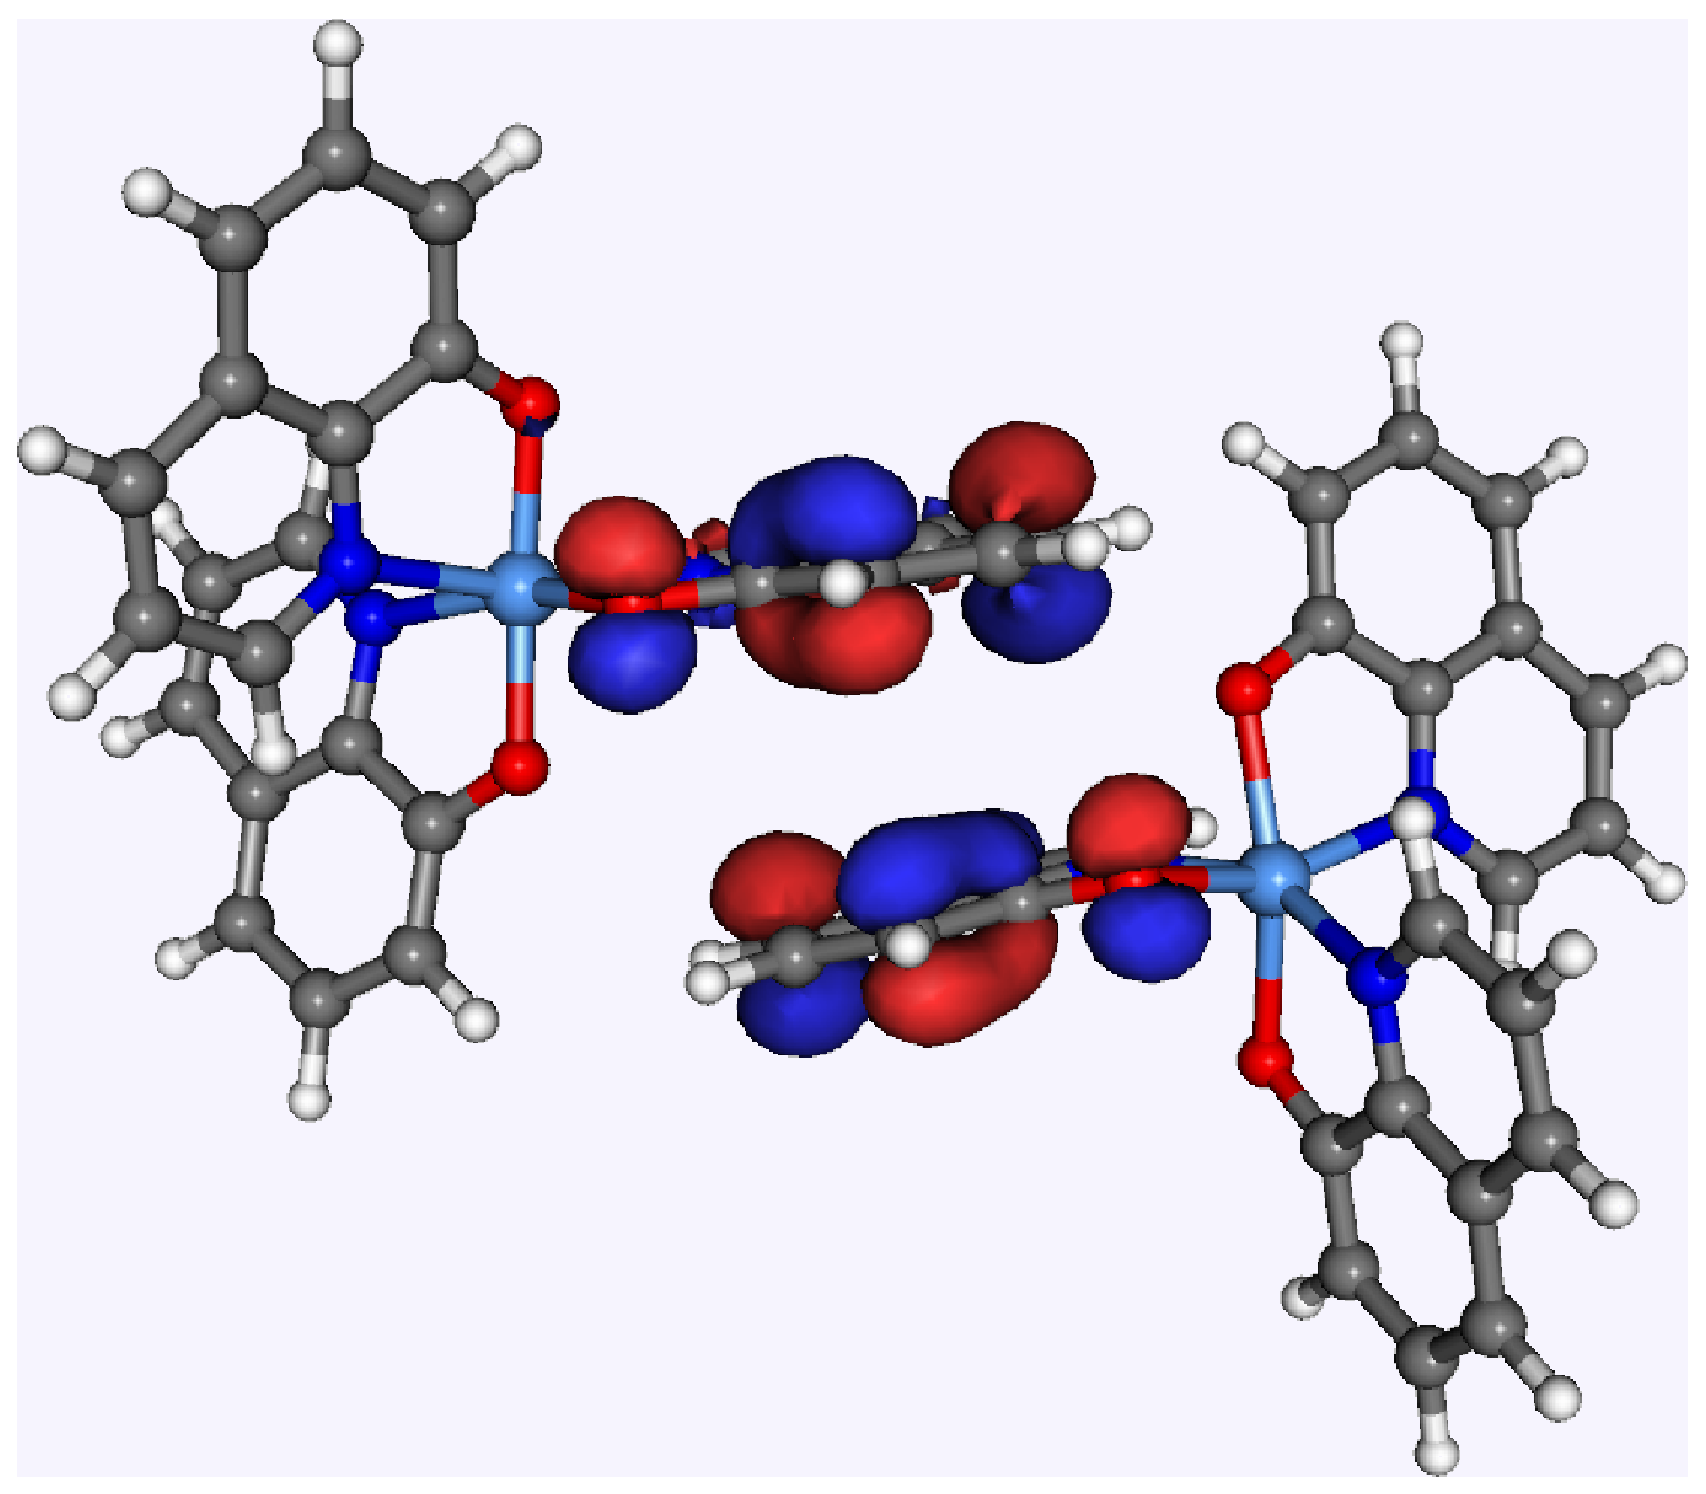
\includegraphics[width=17pt]{fig/logo_trans}}
\newcommand\votcacommand[2]
{
\begin{bclogo}[couleur=mygray, arrondi =0 , logo=\votcalogo, barre=line,noborder=true]{\small #1}
\itshape {\small #2}
\end{bclogo}
}

\newcommand{\xml}{XML\xspace}
\newcommand{\gromacs}{\texttt{GROMACS}\xspace}
\newcommand{\gaussian}{\texttt{Gaussian}\xspace}
\newcommand{\turbomole}{\texttt{Turbomole}\xspace}
\newcommand{\nwchem}{\texttt{NWChem}\xspace}
\newcommand{\tinker}{\texttt{TINKER}\xspace}
\newcommand{\dipro}{\texttt{DIPRO}\xspace}

\newcommand{\Alq}{$\mathrm{Alq}_3$\xspace}
\newcommand{\dcvt}{DCV2T\xspace}

\newcommand{\xyz}{\texttt{geometry.xyz}\xspace}
\newcommand{\orb}{\texttt{zindo.orb}\xspace}
\newcommand{\votcactp}{{\MakeUppercase{votca-ctp}}\xspace}

\newcommand{\calculator}{\hyperref[sec:calculators]{calculator}\xspace}
\newcommand{\tool}{\hyperref[sec:calculators]{tool}\xspace}

\newcommand{\xmloptions}{\texttt{options.xml}\xspace}
\newcommand{\xmlcsg}{\hyperref[sec:xmlmap]{\texttt{map.xml}}\xspace}
\newcommand{\xmlsegments}{\hyperref[sec:xmlsegments]{\texttt{segments.xml}}\xspace}
\newcommand{\sqlstate}{\hyperref[sec:statefile]{\texttt{state.db}}\xspace}
\newcommand{\topology}{\texttt{topol.tpr}\xspace}
\newcommand{\trajectory}{\texttt{traj.xtc}\xspace}

\newcommand{\opt}{\texttt{{ -}o}\xspace}
\newcommand{\seg}{\texttt{{ -}s}\xspace}
\newcommand{\sql}{\texttt{{ -}f}\xspace}
\newcommand{\exe}{\texttt{{ -}e}\xspace}
\newcommand{\tpl}{\texttt{{ -}t}\xspace}
\newcommand{\csg}{\texttt{{ -}m}\xspace}
\newcommand{\trj}{\texttt{{ -}c}\xspace}
\newcommand{\job}{\texttt{{ -}j}\xspace}
\newcommand{\run}{\texttt{{run}}\xspace}
\newcommand{\wrt}{\texttt{{write}}\xspace}
\newcommand{\rd}{\texttt{{read}}\xspace}


\newcommand{\refcalc}{\hyperref[ref:calculators]{calculators}\xspace}

\newcommand{\overlap}{\hyperref[prog:moo_overlap]{\texttt{moo\_overlap}}\xspace}
\newcommand{\ctprun}{\hyperref[prog:ctp_run]{\texttt{ctp\_run}}\xspace}
\newcommand{\ctpmap}{\hyperref[prog:ctp_map]{\texttt{ctp\_map}}\xspace}
\newcommand{\ctpdipro}{\hyperref[prog:ctp_dipro]{\texttt{ctp\_dipro}}\xspace}
\newcommand{\ctpparallel}{\hyperref[prog:ctp_parallel]{\texttt{ctp\_parallel}}\xspace}
\newcommand{\ctpdump}{\hyperref[prog:ctp_dump]{\texttt{ctp\_dump}}\xspace}
\newcommand{\ctpupdate}{\hyperref[prog:ctp_update]{\texttt{ctp\_update}}\xspace}
\newcommand{\ctptools}{\hyperref[prog:ctp_tools]{\texttt{ctp\_tools}}\xspace}
\newcommand{\kmcrun}{\hyperref[prog:kmc_run]{\texttt{kmc\_run}}\xspace}

\newcommand{\sqlite}{\texttt{sqlite3}\xspace}
\newcommand{\sqlconjsegproperties}{\texttt{conjseg\_properties}\xspace}
\newcommand{\sqlconjsegs}{\texttt{conjsegs}\xspace}
\newcommand{\sqlmolecules}{\texttt{molecules}\xspace}
\newcommand{\sqlpairintegrals}{\texttt{pairintegrals}\xspace}
\newcommand{\sqlpairproperties}{\texttt{pairproperties}\xspace}
\newcommand{\sqlpairs}{\texttt{pairs}\xspace}
\newcommand{\sqlrigidfragproperties}{\texttt{rigidfrag\_properties}\xspace}
\newcommand{\sqlrigidfrags}{\texttt{rigidfrags}\xspace}
\newcommand{\sqlframes}{\texttt{frames}\xspace}


\newcommand{\suggestion}[1]{{\color{red}SUGGESTION: #1}}

\newcommand{\segmentref}[1]{segments.#1}
\newcommand{\segmentopt}[1]{\hyperlink{\segmentref{#1}}{\StrSubstitute{#1}{_}{\_}}\xspace}
\newcommand{\calcref}[1]{#1}
\newcommand{\calcopt}[1]{\hyperlink{\calcref{#1}}{\StrSubstitute{#1}{_}{\_}}\xspace}

\newcommand{\calc}[1]{\hyperref[calc:#1]{\texttt{#1}}\xspace}
\newcommand{\toolref}[1]{\hyperref[tool:#1]{\texttt{#1}}\xspace}

\def\bibsection{%
    \chapter*{Bibliography}%
    \addcontentsline{toc}{chapter}{Bibliography}
}

\renewcommand*{\showkeyslabelformat}[1]{{\normalfont\tiny\sffamily#1}}
\definecolor{refkey}{rgb}{1,0,0}
\definecolor{labelkey}{rgb}{1,0,0}

% Calculus and Linear Algbra Notation
% formulas
\newcommand{\vctr}[1]{\mathbf{ \bar{#1} }}
\newcommand{\oper}[1]{\hat{ #1 }}
\newcommand{\matr}[1]{\mathbf{ #1 }}

%% FULL COMMANDS LISTING
\newcommand{\cmdmap}{\ctpmap \tpl \topology \trj \trajectory \seg \xmlcsg  \sql \sqlstate}
\newcommand{\cmdnbl}{\ctprun \opt \xmloptions  \sql  \sqlstate \exe  \calc{neighborlist}}
\newcommand{\cmdemlt}{\ctprun \opt \xmloptions  \sql  \sqlstate \exe  \calc{emultipole}}
\newcommand{\cmdeint}{\ctprun \opt \xmloptions  \sql  \sqlstate \exe  \calc{einternal}}
\newcommand{\cmdedft}{\ctpparallel \opt \xmloptions \sql \sqlstate \exe \calc{edft}}
\newcommand{\cmdidft}{\ctpparallel \opt \xmloptions \sql \sqlstate \exe \calc{idft}}
\newcommand{\cmdizindo}{\ctprun \opt \xmloptions  \sql  \sqlstate \exe  \calc{izindo}}
\newcommand{\cmdouter}{\ctprun \opt \xmloptions  \sql  \sqlstate \exe  \calc{outersphere}}
\newcommand{\cmdrates}{\ctprun \opt \xmloptions  \sql  \sqlstate \exe  \calc{rates}}
\newcommand{\cmdkmc}{ \kmcrun \opt \xmloptions  \sql  \sqlstate \exe  \calc{kmcmultiple}}
\newcommand{\cmdkmcsin}{ \kmcrun \opt \xmloptions  \sql  \sqlstate \exe  \calc{kmcsingle}}
\newcommand{\cmdeana}{\ctprun \opt \xmloptions  \sql  \sqlstate \exe  \calc{eanalyze}}
\newcommand{\cmdmolpol}{\ctptools \opt \xmloptions \exe \toolref{molpol}}
\newcommand{\cmdlogmps}{\ctptools \opt \xmloptions \exe \toolref{log2mps}}
\newcommand{\cmdxqmult}{\ctpparallel \opt \xmloptions \sql \sqlstate \exe \calc{xqmultipole}}



\begin{document}

\addtolength{\oddsidemargin}{0cm}
\addtolength{\evensidemargin}{0cm}
\addtolength{\textwidth}{0cm}
\addtolength{\topmargin}{0cm}
\addtolength{\textheight}{0cm}

\lstset{
  language=XML,
  frame=lines,
  backgroundcolor=\color{invisiblegray},
  basicstyle=\ttfamily\footnotesize,
  identifierstyle=\color{red},
  keywordstyle=\color{blue},
  commentstyle=\color{gray}\rmfamily\itshape,
  mathescape=false
}

\setlength\parindent{0pt}
\frontmatter
\begin{titlepage}

%\center{\fontsize{4cm}{5cm}\selectfont VOTCA-CT}
%\center{\fontsize{1.5cm}{3cm}\selectfont USER MANUAL}

\center{\huge \sc Charge Transport Simulations}
\vspace*{1cm}
\center{\Large \sc User Manual}

\vspace*{3cm}
\center{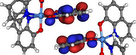
\includegraphics[width=0.6\columnwidth]{fig/logo}}
\vspace*{1cm}

\vfill
{\small% 
If you are using this package please site \\
\vspace*{0.1cm}
V. R\"uhle, A. Lukyanov, F. May, M. Schrader, T. Vehoff, J. Kirkpatrick, B. Baumeier, D. Andrienko \\
``Microscopic simulations of charge transport in disordered organic semiconductors'' \\
\htmladdnormallink{\color{black} {\itshape J. Chem. Theor. Comp.} 2011}
{http://dx.doi.org/} 
%\\
%\vspace*{0.1cm}
%and \\
%\vspace*{0.1cm}
%V. R\"uhle, C. Junghans, A. Lukyanov, K. Kremer, D. Andrienko \\
%``Versatile Object-oriented Toolkit for Coarse-graining Applications'' \\
%\htmladdnormallink{ \color{black} {\itshape J. Chem. Theor. Comp.} 5, 3211, 2009}
%{http://dx.doi.org/10.1021/ct900369w}
}

\vspace*{1.4cm}
\center{\large{\today}}
%\vspace*{-0.3cm}
%\center{\footnotesize{compiled from: \hgid}}
%\center{\footnotesize{Programs version: \refhgid}}

%\vspace*{1cm}
%\center{
%\large{\copyright \hspace*{0.1cm} VOTCA development team}
%}
%\vspace*{0.5cm}



\htmladdnormallink{\color{black}\large{www.votca.org}}{http://www.votca.org}
\end{titlepage}

\thispagestyle{empty}
\cleardoublepage

\tableofcontents
\cleardoublepage
\mainmatter

\printindex
\vfill

\linenumbers

\chapter{Introduction}
\label{sec:introduction}

Charge carrier dynamics in an organic semiconductor can often be described in terms of charge hopping between localized states. The hopping rates depend on \slink{transfer_integrals}{electronic coupling elements}, \slink{reorganization}{reorganization energies}, and \slink{site_energies}{driving forces}, which vary as a function of position and orientation of the molecules.  The exact evaluation of these contributions in a molecular assembly is computationally prohibitive. Various, often semi-empirical, approximations are employed instead. The purpose of the \votcactp package~\cite{ruehle_microscopic_2011} is to simplify the workflow for charge transport simulations, provide a uniform error-control for the methods, flexible platform for their development, and eventually allow in silico prescreening of organic semiconductors for specific applications. 

The toolkit is implemented using modular concepts introduced earlier in the Versatile Object-oriented Toolkit for Coarse-graining Applications (VOTCA)~\cite{ruehle_versatile_2009}. The VOTCA structures are adapted to reading atomistic trajectories, mapping them onto \slink{segments}{conjugated segments and rigid fragments}, and substituting (if needed) rigid fragments with the optimized copies. 

The \slink{izindo}{molecular orbital overlap} module calculates electronic coupling elements between  conjugated segments from the corresponding molecular orbitals. It relies on the semi-empirical INDO Hamiltonian and molecular orbitals in the format provided by the \gaussian package. An alternative,  \slink{dft}{density-functional} based approach, has interfaces to the \gaussian and \turbomole packages. An interface to the \tinker package is provided for calculations of electrostatic and polarization contributions to \slink{site_energies}{energetic disorder}. 

The  \slink{kmc}{kinetic Monte Carlo} module reads in the \slink{neighborlist}{neighbor list}, \slink{morphology}{site coordinates}, and \slink{rates}{hopping rates} and performs charge dynamics simulations using either periodic boundary conditions or charge sources and sinks. 

The toolkit is written as a combination of modular C++ code and scripts. The data transfer between programs is implemented via a \slink{statefile}{state file} (sql database), which is also used to restart simulations. Analysis functions and most of the calculation routines are encapsulated by using the observer pattern~\cite{gamma_design_1995} which allows the implementation of new functions as individual modules.

\chapter{Theoretical background}
\label{sec:theory}

\section{Workflow}
\label{sec:wokflow}

A typical workflow of charge transport simulations is depicted in \fig{workflow}. The first step is the simulation of an \slink{morphology}{atomistic morphology}, which is then partitioned on \slink{segments}{hopping sites}. The coordinates of the hopping sites are used to construct a list of pairs of molecules, or \slink{neighborlist}{neighbor list}. 

\begin{figure}[h]
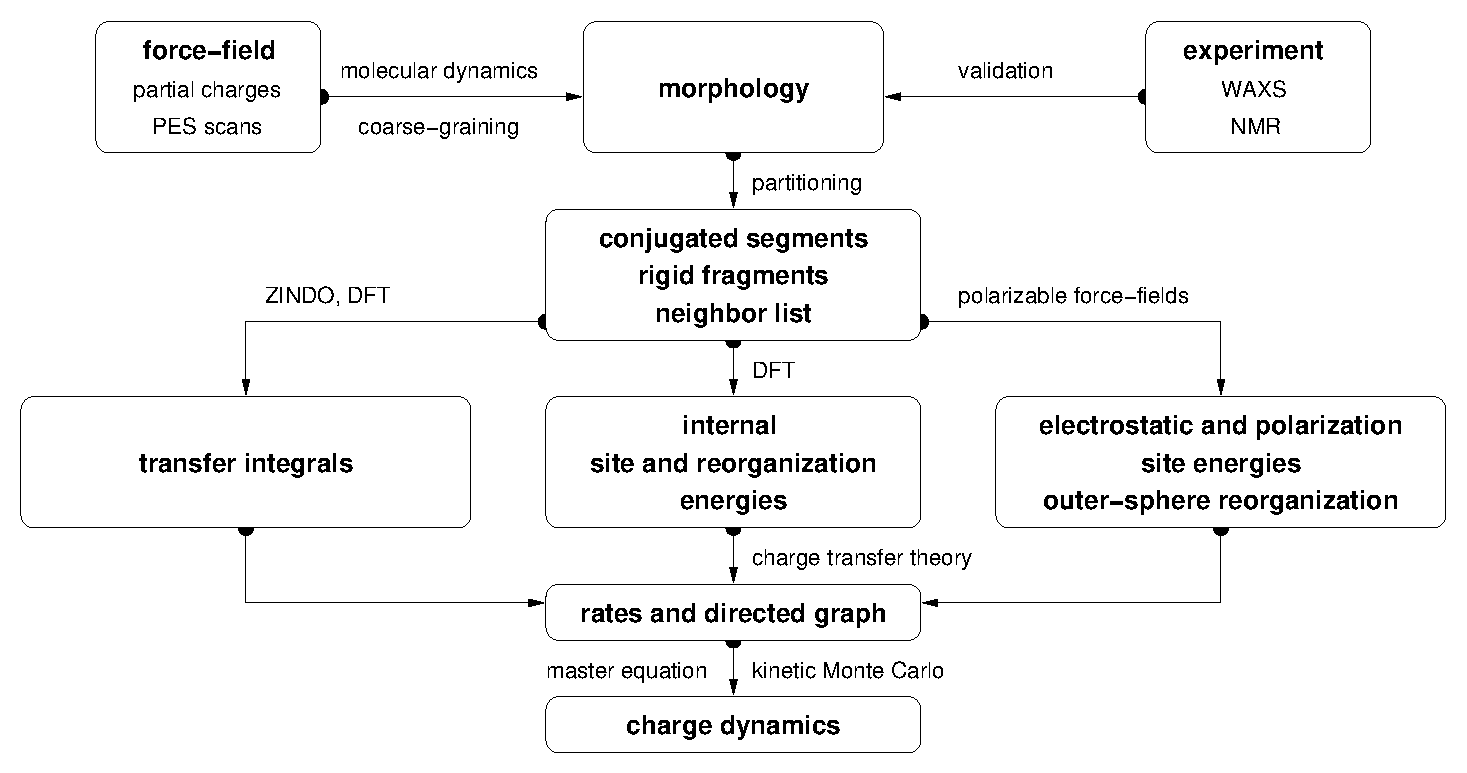
\includegraphics[width=\textwidth]{fig/workflow/workflow}
 \caption{%
   Workflow for microscopic simulations of charge transport.  %
   \label{fig:workflow}}
\end{figure}

For each pair an \slink{transfer_integrals}{electronic coupling element}, a \slink{reorganization}{reorganization energy}, a \slink{site_energies}{driving force}, and eventually the \slink{rates}{hopping rate} are evaluated. The neighbor list and hopping rates define a directed graph. The corresponding master equation is solved using the \slink{kmc}{kinetic Monte Carlo} method, which allows to explicitly monitor the charge dynamics in the system as well as to calculate time or ensemble averages of occupation probabilities, charge fluxes, correlation functions, and field-dependent mobilities.
	
\section{Material morphology}
\label{sec:morphology}

There is no generic recipe on how to predict a large-scale atomistically-resolved morphology of an organic semiconductor. The required methods are system-specific: for ultra-pure crystals, for example, density-functional methods can be used provided the crystal structure is known from experiment. For partially disordered organic semiconductors, however, system sizes much larger than a unit cell  are required. Classical molecular dynamics or Monte Carlo techniques are then the methods of choice. 

In molecular dynamics, atoms are represented by point masses which interact via empirical potentials prescribed by a force-field. Force-fields are parametrized for a limited set of compounds and their refinement is often required for new molecules. In particular, special attention shall be paid to torsion potentials between successive repeat units of conjugated polymers or between functional groups and the $\pi$-conjugated system. First-principles methods can be used to characterize the missing terms of the potential energy function. 

Self-assembling materials, such as soluble oligomers, discotic liquid crystals, block copolymers, partially crystalline polymers, etc., are the most complicated to study. The morphology of such systems often has several characteristic length scales and can be kinetically arrested in a thermodynamically non-equilibrium state. For such systems, the time- and length-scales of atomistic simulations might be insufficient to equilibrate or sample desired morphologies. In this case, systematic coarse-graining can be used to enhance sampling~\cite{ruehle_versatile_2009}. Note that the coarse-grained representation must reflect the structure of the atomistic system and allow for back-mapping to the atomistic resolution.

Here we assume that the morphology is already known, that is we know how the topology and the coordinates of all atoms in the systems at a given time. \votcactp can read standard \gromacs topology files. Custom definitions of \slink{atomistic}{atomistic topology} via \xml files are also possible. Since the description of the atomistic topology is the first step in the charge transport simulations, it is important to follow simple conventions on how the system is partitioned on molecules, residues, and how atoms are named in the topology. Required input files are described in section \slink{atomistic}{atomistic topology}. 

\section{Conjugated segments and rigid fragments}
\label{sec:segments}

\begin{figure}
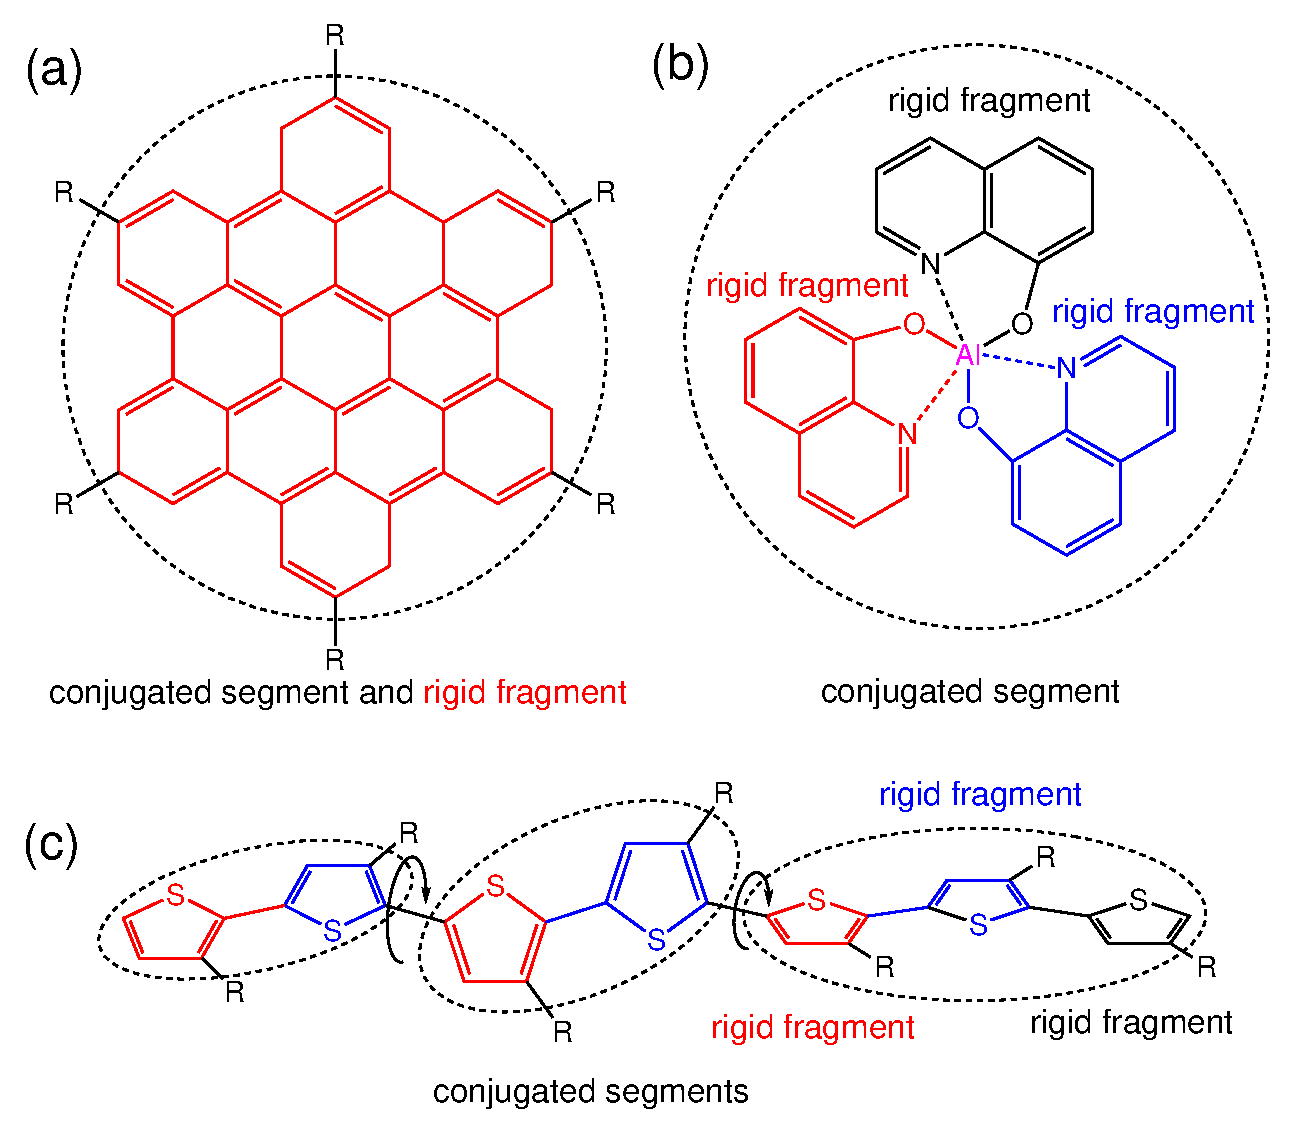
\includegraphics[width=\linewidth]{fig/conjugated_segment/fragment_segment}
\caption{The concept of conjugated segments and rigid fragments. Dashed lines indicate conjugated segments while colors denote rigid fragments. (a) Hexabenzocoronene: the $\pi$-conjugated system is both a rigid fragment and a conjugated segment. (b) \Alq: the Al atom and each ligand are rigid fragments while the whole molecule is a conjugated segment. (c) Polythiophene: each repeat unit is a rigid fragment. A conjugated segment consists of one or more rigid fragments. One molecule can have several conjugated segments.}
\label{fig:segment}
\end{figure}

With the morphology at hand, the next step is partitioning the system on hopping sites\index{hopping site}, or conjugated segments\index{conjugated segment}, and calculating charge transfer rates between them. Physically intuitive arguments can be used for the partitioning,  which reflects the localization of the wave function of a charge. For most organic semiconductors, the molecular architecture includes relatively rigid, planar $\pi$-conjugated systems, which we will refer to as rigid fragments. A conjugated segment can contain one or more of such rigid fragments, which are linked by bonded degrees of freedom. The dynamics of these degrees of freedom evolves on timescales much slower than the frequency of the internal promoting mode. In some cases, e.g. glasses, it can be `frozen' due to non-bonded interactions with the surrounding molecules.

To illustrate the concept of conjugated segments and rigid fragments, three representative molecular architectures are shown in \fig{segment}. The first one is a typical discotic liquid crystal, hexabenzocoronene. It consists of a conjugated core to which side chains are attached to aid self-assembly and solution processing. In this case the orbitals localized on side chains do not participate in charge transport and the conjugated $\pi$-system is both, a rigid fragment and a conjugated segment. 
%
In \Alq, a metal-coordinated compound, a charge carrier is delocalized over all three ligands. Hence, the whole molecule is one conjugated segment. Individual ligands are relatively rigid, while energies of the order of $k_\text{B}T$ are sufficient to reorient them with respect to each other. Thus the Al atom and the three ligands are rigid fragments.
%
In the case of a conjugated polymer, one molecule can consist of several conjugated segments, while each backbone repeat unit is a rigid fragment. Since the conjugation along the backbone can be broken due to large out-of-plane twists between two repeat units, an empirical criterion, based on the dihedral angle, can be used to partition the backbone on conjugated segments~\cite{ruhle_multiscale_2010}. However, such intuitive partitioning is, to some extent, arbitrary and shall be validated by other methods~\cite{vukmirovic_charge_2008,vukmirovic_charge_2009,mcmahon_ad_2009}. 

After partitioning, an additional step is often required to remove bond length fluctuations introduced by molecular dynamics simulations, since they are already integrated out in the derivation of the rate expression. This is achieved by substituting respective molecular fragments with  rigid, planar $\pi$-systems\index{rigid fragment} optimized using first-principles methods. Centers of mass and gyration tensors are used to align rigid fragments, though a custom definition of local axes is also possible. Such a procedure also minimizes discrepancies between the force-field and first-principles-based ground state geometries of conjugated segments, which might be important for calculations of electronic couplings, reorganization energies, and intramolecular driving forces. 

To partition the system on hopping sites and substitute rigid fragments with the corresponding ground-state geometries \ctpmap program is used:
\votcacommand{Mapping the \gromacs trajectory}{\cmdmap}
It reads in the \gromacs topology (\topology) and trajectory (\trajectory) files, definitions of conjugated segments and rigid fragments (\xmlcsg) and outputs coordinates of conjugated segments (hopping sites) and rigid fragments (as provided in the MD trajectory and after rigidification) to the  state file (\sqlstate). In order to do this, a mapping file \xmlcsg has to be provided, which specifies the corresponding atoms in the different representations. After this step, all information (frame number, dimensions of the simulation box, etc) are stored in the \slink{statefile}{state file} and only this file is used for further calculations.

\attention{\votcactp requires a wrapped trajectory for mapping the segments and fragments, so all molecules should be whole in the frame.}   

In order to visually check the mapping one can use either the \calc{tdump} \calculator or the programm \ctpdump with the calculator \calc{trajectory2pdb}.

\label{sec:ctp_dump}
\votcacommand{Writing a mapped trajectroy with \ctpdump}{\small \ctpdump \sql \sqlstate \exe \calc{trajectory2pdb} }

It reads in the state file created by \ctpmap and outputs two trajectory files corresponding to the original and rigidified atom coordinates. To check the mapping, it is useful to superimpose the three outputs (original atomistic, atomistic stored in the state file, and rigidified according to ground state geometries), e.g., with {\tt VMD}.

\label{sec:tdump}
\votcacommand{Writing a mapped trajectroy with \calc{tdump} }{\small \ctprun \sql \sqlstate \opt \xmloptions \exe \calc{tdump} }

It also reads in the state file but appends the coordinates to a pdb. file. So make sure to delete old QM.pdb and MD.pdb if you want to create a new imagef



\section{Neighbor list}
\label{sec:neighborlist}

A list of neigboring conjugated segments, or neighbor list\index{neighbor list}, contains all pairs of conjugated segments for which \slink{sec:transfer_integrals}{coupling elements}, \slink{sec:reorganization}{reorganization energies}, \slink{sec:site_energies}{site energy differences}, and \slink{sec:rates}{rates} are evaluated.

Two segments are added to this list if the distance between centers of mass of any of their rigid fragments is below a certain cutoff. This allows neighbors to be selected on a criterion of minimum distance of approach rather than center of mass distance, which is useful for molecules with anisotropic shapes.

The neighbor list can be generated from the atomistic trajectory by using the \calc{neighborlist} \calculator. This calculator requires a cutoff, which can be specified in the \xmloptions file. The list is saved to the \sqlstate file:
\votcacommand{Generating a neighbor list}{\cmdnbl}

\section{Reorganization energy}
\label{sec:reorganization}

The reorganization energy\index{reorganization energy} $\lambda_{ij}$ takes into account the change in  nuclear (and dielectric) degrees of freedom as the charge moves from donor $i$ to acceptor $j$. It has two contributions: intramolecular, $\lambda^\text{int}_{ij}$, which is due to reorganization of nuclear coordinates of the two molecules forming the charge transfer complex, and intermolecular (outersphere), $\lambda^\text{out}_{ij}$, which is due to the relaxation of the nuclear coordinates of the environment. In what follows we discuss how these contributions can be calculated.

\subsection{Intramolecular reorganization energy}
\label{sec:inner_reorganization}
\index{reorganization energy!intramolecular}
If intramolecular vibrational modes of the two molecules are treated classically, the rearrangement of their nuclear coordinates after charge transfer results in the dissipation of the internal reorganization energy, $\lambda_{ij}^\text{int}$. It can be computed from four points on the potential energy surfaces (PES) of both molecules in neutral and charged states, as indicated in \fig{parabolas}. 

\begin{figure}
   \centering
   \includegraphics[width=0.7\linewidth]{fig/reorganization_energy/monomer_parabolas}
    \caption{Potential energy surfaces of (a) donor and (b) acceptor in charged and neutral states. After the change of the charge state both molecules relax their nuclear coordinates. If all vibrational modes are treated classically, the total internal reorganization energy and the internal energy difference of the electron transfer reaction are $\lambda_{ij}^\text{int} = \lambda_{i}^\text{cn} + \lambda_{j}^\text{nc}$ and $\Delta E_{ij}^\text{int} =  \Delta U_i - \Delta U_j$, respectively.}
   \label{fig:parabolas}
\end{figure}


Adding the contributions due to discharging of molecule $i$ and charging of molecule $j$ yields~\cite{bredas_charge-transfer_2004}
\begin{equation}
\lambda_{ij}^\text{int} =\lambda_{i}^{cn}+\lambda_{j}^{nc}=U_{i}^{nC}-U_{i}^{nN}+U_{j}^{cN}-U_{j}^{cC}\,.
\label{equ:lambdas}
\end{equation}
Here $U_{i}^{nC}$ is the internal energy of the neutral molecule $i$ in the geometry of its charged state (small $n$ denotes the state and capital $C$ the geometry). Similarly, $U_{j}^{cN}$ is the energy of the charged molecule $j$ in  the geometry of its neutral state.
%If the PES of neutral and charged states are different for the same molecule, that is  $\lambda^{cn}_i \neq \lambda^{nc}_i$, the rate for the bimolecular charge transfer is no longer a simple sum. If, as before, both modes are treated classically, the rate is an integral over the charge detachment and attachment spectrum of molecules $i$ and $j$~\cite{kakitani_comprehensive_1987}. For most systems, however, the reorganization energies for charging or discharging of the same molecule do not deviate by more than a few percent and the rate is given by~\equ{marcus}.
%
Note that the PES of the donor and acceptor are not identical for chemically different compounds or for conformers of the same molecule. In this case $\lambda_{i}^{cn} \ne \lambda_{j}^{cn}$ and  $\lambda_{i}^{nc} \ne \lambda_{j}^{nc}$. Thus $\lambda_{ij}^\text{int}$ is a property of the charge transfer complex, and not of a single molecule.

Intramolecular reorganization energies for discharging ($\lambda^{cn}$) and charging ($\lambda^{nc}$) of a molecule are provided in the \xmlsegments file and are written to the \sqlstate file by the \ctpmap program. 

\subsection{Outersphere reorganization energy}
\index{reorganization energy!outersphere}
\label{sec:outer_reorganization}
During the charge transfer reaction, also the molecules outside the charge transfer complex reorient and polarize in order to adjust for changes in electric potential, resulting in the outersphere contribution to the reorganization energy. $\lambda_{ij}^\text{out}$ is particularly important if charge transfer occurs in a polarizable environment. Assuming that charge transfer is much slower than electronic polarization but much faster than nuclear rearrangement of the environment, $\lambda_{ij}^\text{out}$ can be calculated from the electric displacement fields created by the charge transfer complex~\cite{may_charge_2003}
\begin{equation}
\lambda_{ij}^\text{out}=
\frac{c_p}{2\epsilon_0}\int_{V^\text{out}}d V
\left[ \vec{D}_I(\vec{r}) - \vec{D}_F(\vec{r}) \right]^2\,,
\label{equ:lambda_outer1}
\end{equation}
where $\epsilon_0$ is the the permittivity of free space, $\vec{D}_{I,F}(\vec{r})$ are the electric displacement fields created by the charge transfer complex in the initial (charge on molecule $i$) and final (charge transferred to molecule $j$) states,  $V^\text{out}$ is the volume outside the complex, and $c_p=\frac{1}{\epsilon_\text{opt}}-\frac{1}{\epsilon_\text{s}}$ is the Pekar factor, which is determined by the low ($\epsilon_\text{s}$) and high ($\epsilon_\text{opt}$) frequency dielectric permittivities.

\Equ{lambda_outer1} can be simplified by assuming spherically symmetric charge distributions on molecules $i$ and $j$ with total charge $e$. Integration over the volume $V^\text{out}$ outside of the two spheres of radii $R_i$ and $R_j$ centered on molecules $i$ and $j$ leads to the classical Marcus expression for the outersphere reorganization energy
\begin{equation}
\lambda_{ij}^\text{out}=\frac{c_{p}e^2}{4\pi\epsilon_0}\left(\frac{1}{2 R_i}+\frac{1}{2 R_j}-\frac{1}{r_{ij}} \right)\,,
\label{equ:lambda_outer2}
\end{equation}
where $r_{ij}$ is the molecular separation.  While \equ{lambda_outer2} captures the main physics, e.g. predicts smaller outer-sphere reorganization energies (higher rates) for molecules at smaller separations, it often cannot provide quantitative estimates, since charge distributions are rarely spherically symmetric. 

Alternatively, the displacement fields can be constructed using the atomic partial charges. The difference of the displacement fields at the position of an atom $b_k$ outside the charge transfer complex (molecule $k \ne i,j$)  can be expressed as
\begin{eqnarray}
\label{equ:disp_atom}
\vec{D}_I(\vec{r}_{b_k}) - \vec{D}_F(\vec{r}_{b_k})  = 
\sum_{a_i} \frac{q_{a_i}^c - q_{a_i}^n}{4\pi } \frac{ (\vec{r}_{b_k} - \vec{r}_{a_i} ) }
                                            {|\vec{r}_{b_k}-\vec{r}_{a_i}|^3}+
\sum_{a_j} \frac{q_{a_j}^n - q_{a_j}^c}{4\pi } \frac{ (\vec{r}_{b_k}-\vec{r}_{a_j} ) } 
                                            {|\vec{r}_{b_k}-\vec{r}_{a_j}|^3}\,,
%\nonumber
\end{eqnarray}
where $q^n_{a_i}$ ($q^c_{a_i}$) is the partial charge of atom $a$ of the neutral (charged) molecule $i$ in vacuum. The partial charges of neutral and charged molecules are obtained by fitting their values to reproduce the electrostatic potential of a single molecule (charged or neutral) in vacuum. 
%
Assuming a uniform density of atoms, the integration in~\equ{lambda_outer1} can be rewritten as a density-weighted sum over all atoms excluding those of the charge transfer complex.

The remaining unknown needed to calculate $\lambda_{ij}^\text{out}$ is the Pekar factor\index{Pekar factor}, $c_p$. In polar solvents $\epsilon_\text{s}\gg\epsilon_\text{opt}\sim 1$ and $c_p$ is of the order of 1. In most organic semiconductors, however, molecular orientations are fixed and therefore the low frequency dielectric permittivity is of the same order of magnitude as $\epsilon_\text{opt}$. Hence, $c_p$ is small and its value is very sensitive to differences in the permittivities. 


Outersphere reorganization energies for all pairs of molecules in the \slink{neighborlist}{neighbor list} can be computed from the atomistic trajectory by using the \calc{eoutersphere} \calculator. 

Two methods can be used to compute $\lambda_{ij}^\text{out}$. The first method uses the atomistic partial charges of neutral and charged molecules from files specified in \xmlsegments and \equ{lambda_outer1}. The Pekar factor $c_p$ and a cutoff radius  based on molecular centers of mass have to be specified in the \xmloptions file. 

If this method is computationally prohibitive, $\lambda_{ij}^\text{out}$ can be computed using \equ{lambda_outer2}, which assumes spherical charge distributions on the molecules. In this case the radii of these spheres are specified in \xmlsegments, while the Pekar factor $c_p$ is given in the \xmloptions file and no cutoff radius is needed. 

The outer sphere reorganization energies are saved to the \sqlstate file:

{\small \ctprun \opt \xmloptions  \seg  \xmlsegments \sql  \sqlstate \exe  \calc{eoutersphere}}

\section{Site energies}
\label{sec:site_energies}
A charge transfer reaction between molecules $i$ and $j$ is driven by the site energy\index{site energy} difference, $\Delta E_{ij} = E_i - E_j$. Since the  transfer rate, $\omega_{ij}$, depends exponentially on $\Delta E_{ij}$ (see~\equ{marcus}) it is important to compute its distribution as accurately as possible.  The total site energy difference has contributions due to \slink{ext_field}{externally applied electric field}, \slink{ecoulomb}{electrostatic interactions}, polarization effects, and \slink{internal_energy}{internal energy} differences. In what follows we discuss how to estimate these contributions by making use of first-principles calculations and polarizable force-fields.

\subsection{Externally applied electric field}
\label{sec:ext_field}
The contribution to the total site energy\index{site energy!external field} difference due to an external electric field $\vec{F}$ is given by $\Delta E_{ij}^\text{ext} = q {\vec{F} \cdot \vec{r}_{ij}}$, where $q=\pm e$ is the charge and $\vec{r}_{ij} = \vec{r}_i  - \vec{r}_j $ is a vector connecting molecules $i$ and $j$. For typical distances between small molecules, which are of the order  of $1\,\unit{nm}$, and moderate fields of $F<10^8\,\unit{V/m}$ this term is always smaller than $0.1\, \unit{eV}$.

\subsection{Electrostatic energy}
\label{sec:ecoulomb}
\index{site energy!electrostatic}

Variations of the local electric field can result in large electrostatic contributions to the energetic disorder. Using the atomic partial charges of charged and neutral molecules, $\Delta E_{ij}^\text{el}$ can be computed from the site energies~\cite{kirkpatrick_columnar_2008}
\begin{equation}
E_{i}^\text{el}  = \frac{1}{4 \pi \epsilon_0} \sum_{a_i} \sum_{\substack{b_k   \\ k\neq i }}
\frac{ \left( q^c_{a_i} - q^n_{a_i} \right) q^n_{b_k}}{ \epsilon_\text{s} r_{a_i b_k}} 
\, ,
\label{equ:estatic}
\end{equation}
where $r_{a_i b_k}=|\vec{r}_{a_i} - \vec{r}_{b_k}|$ is the distance between atoms $a_i$ and $b_k$,   $\epsilon_\text{s}$ is the static relative dielectric constant.
%
The first sum extends over all atoms of molecule $i$, for which the site energy is calculated. The second sum reflects interactions with all atoms of neutral molecules $k \ne i$. By using \equ{estatic}, one assumes that the influence of conformational changes on partial charges and changes of the molecular geometry upon charging are small. In order to minimize finite size effects, we do not use spherical cutoff but apply the nearest image convention, that is sum over all neutral molecules in the box after centering the box around the charged molecule. 

The influence of polarization effects on the Coulomb interactions can be taken into account by using a relative dielectric constant in \equ{estatic}. Bulk values of  $\epsilon_\text{s} = 2-5$ for typical organic semiconductors uniformly scale all site energies but are not capable of describing polarization effects on a microscopic level. 
The contribution to $E_i^\text{el}$ from the first coordination shell is then underestimated due to overscreening and, as a result, the site-energy differences become artificially small. Alternatively, one can introduce a phenomenological distance-dependent screening function $\epsilon(r_{a_i b_k})$ in~\equ{estatic}~\cite{nagata_atomistic_2008}
\begin{equation}
\epsilon(r)=\epsilon_{\text{s}} - (\epsilon_{\text{s}} - 1)
\left( 1 + sr + \frac{1}{2}s^2r^2 \right) 
\mathrm{e}^{ -sr}\,,
\label{equ:epss}
\end{equation}
where the parameter $s$ is the inverse screening length. For a monovalent ion in water, for example, $\epsilon_{\text{s}}=80$ and $s=3\,\textrm{nm}^{-1}$~\cite{daggett_molecular_1991}. This screening function ensures that neighboring atoms interact via an unscreened Coulomb potential ($\epsilon \sim 1$) while the electrostatic interaction between atoms at large separations is screened as in the bulk. 

Evaluation of the electrostatic contribution is provided by the \calc{ecoulomb} \calculator. Atomistic partial charges for charged an neutral molecule are taken from files specified in the \xmlsegments files. Note that, in order to speed up calculations for both methods, a cutoff radius (for the molecular centers of mass) can be given in  \xmloptions.

The electrostatic site energies are saved to the \sqlstate file:

{\noindent \small \ctprun \opt \xmloptions  \sql  \sqlstate \exe  \calc{ecoulomb} }

\subsection{Internal energy difference}
\label{sec:internal_energy}

The contribution to the site energy difference due to different internal energies\index{site energy!internal} (see \fig{parabolas}) can be written as
\begin{equation}
 \Delta E_{ij}^\text{int}=
\Delta U_i - \Delta U_j = \left( U_{i}^{cC}-U_{i}^{nN}\right) - \left( U_{j}^{cC}-U_{j}^{nN}\right) \, ,
\label{equ:conformational}
\end{equation}
where $U_{i}^{cC(nN)}$ is the total energy of molecule $i$ in the charged (neutral) state and geometry.  $\Delta U_{i}$ corresponds to the adiabatic ionization potential (or electron affinity) of molecule $i$, as shown in~\fig{parabolas}. For one-component systems and negligible conformational changes $ \Delta E_{ij}^\text{int}=0$, while it is significant for donor-acceptor systems.

\subsection{Electrostatic interaction energy}
\label{sec:distributed_multipoles}
\index{distributed multipoles}
\index{site energy!distributed multipoles}

We represent the molecular charge density by choosing multiple expansion sites (``polar sites'') per molecule in such a way as to accurately reproduce the molecular electrostatic potential (ESP), with a set of suitably chosen multipole moments $\{Q_{lk}^a\}$ (in spherical-tensor notation) allocated to each site. The expression for the electrostatic interaction energy between two molecules $A$ and $B$ in the multi-point expansion includes an implicit sum over expansion sites $a\epsilon A$ and $b\epsilon B$,
\begin{align}
 U_{AB} & = \sum_{a\epsilon A} \sum_{b\epsilon B} \hat{Q}_{l_1k_1}^a T_{l_1k_1l_2k_2}^{a,b} \hat{Q}_{l_2k_2}^b \equiv  \hat{Q}_{l_1k_1}^a T_{l_1k_1l_2k_2}^{a,b} \hat{Q}_{l_2k_2}^b,
 \label{equ:mol_distributed_U}
\end{align}
where we have used the Einstein sum convention for the site indices $a$ and $b$ on the right-hand side of the equation, in addition to the sum convention that is in place for the multipole-moment components $t\equiv l_1 k_1$ and $u\equiv l_2 k_2$. The $T_{l_1k_1l_2k_2}^{a,b}$ are tensors that mediate the interaction between a multipole component $l_1 k_1$ on site $a$ with the moment $l_2 k_2$ on site $b$. If we include the molecular environment into a perturbative term $W$ to enter in the single-molecule Hamiltonian, the above expression is exactly the first-order correction to the energy where the quantum-mechanical detail has been absorbed in classical multipole moments.

The are a number of strategies how to arrive at such a collection of {\em distributed multipoles}. They can be classified according to whether the multipoles are derived (a) from the electrostatic potential generated by the SCF charge density or (b) from a decomposition of the wavefunction itself. Here, we will only draft two of those approaches, CHELPG~\cite{breneman_determining_1990} from category (a) and DMA~\cite{stone_distributed_1985} from category (b).

The CHELPG (CHarges from ELectrostatic Potentials, Grid-based) method relies on performing a least-squares fit of atom-placed charges to reproduce the electrostatic potential as evaluated from the SCF density on a regularly spaced grid~\cite{breneman_determining_1990}. The fitted charges result from minimizing the Lagrangian function~\cite{chirlian_atomic_1987}
\begin{align}
 z(\{q_i\}) = \sum_{k=1}^M \left( \phi(\vec{r}_k) - \sum_{i=1}^N \frac{1}{4\pi\varepsilon_0} \frac{q_i}{|\vec{r}_i-\vec{r}_k|} \right) + \lambda \left( q_\textrm{mol} - \sum_{i=1}^N q_i \right),
\end{align}
with $M$ grid points, $N$ atomic sites, the set of atomic partial charges $\{q_i\}$ and the SCF potential $\phi$. The Lagrange multiplier $\lambda$ constrains the sum of the fitted charges to the molecular charge $q_\textrm{mol}$. The main difference from other fitting schemes~\cite{singh_approach_1984} is the algorithm that selects the positions at which the potential is evaluated (we note that the choice of grid points can have substantial effects especially for bulky molecules).
Clearly, the CHELPG method can be (and has been) extended to include higher atomic multipoles. It should be noted, however, how already the inclusion of atomic dipoles hardly improves the parametrization, and can in fact be harmful to its conformational stability.

The Distributed-Multipole-Analysis (DMA) approach~\cite{stone_distributed_1985, stone_distributed_2005}, developed by A. Stone, operates directly on the quantum-mechanical density matrix, expanded in terms of atom- and bond-centered Gaussian functions $\chi_\alpha = R_{LK}(\vec{x}-\vec{s}_\alpha) \exp[-\zeta(\vec{x}-\vec{s}_\alpha)^2]$,
\begin{align}
 \rho(\vec{x}) = \sum_{\alpha,\beta} \rho_{\alpha\beta} \chi_\alpha(\vec{x}-\vec{s}_\alpha) \chi_\beta(\vec{x}-\vec{s}_\beta). 
\end{align}
The aim is to compute multipole moments according in a distributed fashion: If we use that the overlap product $\chi_\alpha \chi_\beta$ of two Gaussian basis functions yields itself a Gaussian centered at $\vec{P} = (\zeta_\alpha \vec{s}_\alpha + \zeta_\beta \vec{s}_\beta) / (\zeta_\alpha + \zeta_\beta)$, it is possible to proceed in two steps: First, we compute the multipole moments associated with a specific summand in the density matrix, referred to the overlap center $\vec{P}$:
\begin{align}
 Q_{LK}[\vec{P}] = - \int R_{LK}(\vec{x}-\vec{P}) \rho_{\alpha\beta} \chi_\alpha \chi_\beta d^3\!x.
\end{align}
Second, we transfer the resulting $Q_{lk}[\vec{P}]$ to the position $\vec{S}$ of a polar site according to the rule~\cite{stone_distributed_1985}
\begin{align}
 Q_{nm}[\vec{S}] = \sum_{l=0}^L \sum_{k=-l}^l \left[ \left(\begin{array}{c} n+m \\ l+k \end{array}\right)\left(\begin{array}{c} n-m \\ l-k \end{array}\right) \right]^{1/2} R_{n-l,m-k}(\vec{S}-\vec{P})\cdot Q_{lk}[\vec{P}].
\end{align}
Note how this requires a rule for the choice of the expansion site to which the multipole moment should be transferred. In the near past~\cite{stone_distributed_2005}, the nearest-site algorithm, which allocates the multipole moments to the site closest to the overlap center, was replaced for diffuse functions by an algorithm based on a sxtpth weighting function in conjunction with grid-based integration methods in order to decrease the basis-set dependence of the resulting set of distributed multipoles.

One important advantage of the DMA approach over fitting algorithms such as CHELPG or Merz-Kollman (MK) is that higher-order moments can also be derived without too large an ambiguity.

The `mps' file format used by VOTCA for the definition of distributed multipoles (as well as point polarizabilities, see subsequent section) is based on the GDMA punch format of A. Stone's GDMA program~\cite{stone_distributed_2005} (the punch output file can be immediately plugged into VOTCA without any conversions to be applied). Furthermore the log-file of different QM packages (currently \gaussian, \turbomole and \nwchem) may be fed into the \toolref{log2mps} \tool, which will subsequently generate the appropriate mps-file.

\votcacommand{Read in ESP charges from a QM log file}{\cmdlogmps}
\subsection{Thole model}
See the following reference for details~\cite{thole_molecular_1981}.
\section{Electronic coupling elements}
\label{sec:transfer_integrals}

The electronic transfer integral\index{electronic coupling} element $J_{ij}$ entering the Marcus rates in \equ{marcus} is defined as
\begin{equation}
   J_{ij} = \left\langle \phi^i \left\vert \hat{H} \right\vert \phi^j \right\rangle ,
\label{equ:TI}
\end{equation}
where $\phi^i$ and $\phi^j$ are diabatic wavefunctions, localized on molecule $i$ and $j$ respectively, participating in the charge transfer, and $\hat{H}$ is the Hamiltonian of the formed dimer. Within the frozen-core approximation, the usual choice for the diabatic wavefunctions $\phi^i$  is the highest occupied molecular orbital (HOMO) in case of hole transport, and the lowest unoccupied molecular orbital (LUMO) in the case of electron transfer, while $\hat{H}$ is an effective single particle Hamiltonian, e.g. Fock or Kohn-Sham operator of the dimer. As such, $J_{ij}$ is a measure of the strength of the electronic coupling of the frontier orbitals of monomers mediated by the dimer interactions. Intrinsically, the transfer integral is very sensitive to the molecular arrangement, i.e. the distance and the mutual orientation of the molecules participating in charge transport. Since this arrangement can also be significantly influenced by
static and/or dynamic disorder~\cite{hutchison_hopping_2005,kirkpatrick_columnar_2008,troisi_charge_2009,vehoff_charge_2010-1,vehoff_charge_2010-2},
it is essential to calculate $J_{ij}$ explicitly for each hopping pair within a realistic morphology. Considering that the number of dimers for which \equ{TI} has to be evaluated is proportional to the number of molecules times their coordination number, computationally efficient and at the same time quantitatively reliable schemes are required.

In general, information about three objects is needed: the two monomer wave functions $\phi^i$ and $\phi^j$, and the dimer interaction Hamiltonian $\hat{H}$.  

\newcommand{\integrals}{\hyperref[calc:integrals]{\texttt{integrals}}\xspace}

\subsection{Molecular Orbital Overlap}

\moo can be used both in a sandalone mode and as a \calculator of the \votcact. \moo constructs the Fock operator of a dimer from the  molecular orbitals of monomers by translating and rotating the orbitals and therefore requires the optimized geometry of the molecule and the projection coefficients of the molecular on atomic orbitals. 


\subsubsection{Standalone mode}
For a standalone mode program \overlap is provided 
\begin{verbatim}
 moo_overlap --conjseg benzene.xml --pos1 benzene1.pos --pos2 benzene2.pos
\end{verbatim}
Its input requires a description of two conjugated segments (\texttt{benzene.xml}, positions and orientations of the molecules and the files with molecular coordinates and orbitals. The structure of the files is shown in listings \ref{list:benzene_xml} and  \ref{list:benzene_pos}.
\vskip 0.1cm
\lstinputlisting[label=list:benzene_xml,caption={\small \texttt{benzene.xml} file with the description of the benzene molecule, which is also a single conjugated segment and a rigid fragment.}] {./fig/moo/moo_overlap/benzene.xml}
\vskip 0.1cm
\lstinputlisting[label=list:benzene_pos, caption={\small \texttt{benzene1.pos} file which describes the position and orientation of the molecule. The name of the molecule is followed by three coordinates (relative to the center of mass of the supplied \texttt{xyz} file and then by nine elements of the rotation matrix $a_{ij} = e_i e^\text{mol}_j $. The reference coordinate frame is determined from the provided \texttt{xyz} file.}] {./fig/moo/moo_overlap/benzene1.pos}


\subsubsection{Calculator of \votcact}
Semi-empirical method of evaluation of electronic couplings is provided by the \integrals \calculator.


\moo requires the following input files: \\
\noindent
\xyz contains four columns, first being the atom type and the next three its coordinates. This is a standard \texttt{xyz} format without a header. 
\vskip 0.1cm
\noindent

\subsubsection{Molecular orbitals}
\orb can be generated using \gaussian program and the input script \texttt{get\_orbitals.com} which shown in listing~\ref{list:zindo_orbitals}.
\vskip 0.1cm
\noindent
\lstinputlisting[
 label=list:zindo_orbitals, 
 caption={\footnotesize \gaussian input file \texttt{get\_orbitals.com} used for generating molecular orbitals. The first line contains  the name of the check file, the second the requested RAM. 
%
 \texttt{int=zindos} requests the method ZINDO, \texttt{punch=mo} states that the molecular orbitals ought to be written to  the \texttt{fort.7} file, \texttt{nosymm} forbids use of symmetry and is necessary to ensure correct position of orbitals with respect to the provided coordinates. The two integer numbers correspond to the charge and multiplicity of the system: $0\, 1$ corresponds to a neutral system with a multiplicity of one. They are followed by the types and coordinates of all atoms in the molecule.
}]%
{./fig/moo/get_orbitals.com}
%
Provided with this input, \gaussian will generate \texttt{fort.7} file containing the molecular orbitals of a single molecule. This file can be renamed to \orb. 


\subsection{Density-functional method}
\label{sec:dft}

\begin{itemize}
\item {\it not sure about directory structure yet, using {\tt
      \$DIRECTORY} for the time being}
\item creating file structure for frame $N$ (raw: no postpocessing,
  min: MD energy minimization) in directory {\tt OUTDIR}
\begin{verbatim}
$DIRECTORY/perpare.sh raw/min N OUTDIR
cd OUTDIR
$DIRECTORY/pairdump.sh
\end{verbatim}
\item make sure QCP environments are set!
\item running calculations for all monomers
 \begin{verbatim}
$DIRECTORY/calc_monomer QCP [METHOD]

QCP:   G for Gaussian09
       T for Turbomole

METHOD: func/basis (optional)
        overrides default functional/basisset combination
        defaults: pbepbe/6-311G** Gaussian09
                  b-p/def-TZVP    Turbomole
\end{verbatim}
\item check monomer calculations (Gaussian version to test!) 
\begin{verbatim}
$DIRECTORY/check_mols N M QCP

N:   First monomer to test
M:   Last monomer to test
QCP: G/T 
\end{verbatim}
incomplete monomers are written to file {\tt TROUBLE.mol}
\item running calculations for all dimers
 \begin{verbatim}
$DIRECTORY/calc_dimer_noSCF QCP [METHOD]

QCP:   G for Gaussian09
       T for Turbomole

METHOD: func/basis (optional)
        overrides default functional/basisset combination
        defaults: pbepbe/6-311G** Gaussian09
                  b-p/def-TZVP    Turbomole
\end{verbatim}
\item should we add {\tt trajectory\_submit.sh} that does all monomer
  and dimer calculations on the cluster (MPIP-specific)?
\end{itemize}


\section{Charge transfer rate}
\label{sec:rates}

Charge transfer rates\index{charge transfer rate} can be postulated based on intuitive physical considerations, as it is done in the Gaussian disorder models~\cite{walker_electrical_2002,baessler_charge_1993,borsenberger_charge_1991,pasveer_unified_2005}. Alternatively, charge transfer theories can be used to evaluate rates from quantum chemical calculations~\cite{bredas_molecular_2009,coropceanu_charge_2007,bredas_charge-transfer_2004,nelson_modeling_2009,baumeier_density-functional_2010,ruhle_microscopic_2011}. In spite of being significantly more computationally demanding, the latter approach allows to link the chemical and electronic structure, as well as the morphology, to charge dynamics.

\subsection{Classical charge transfer rate}
\label{sec:rate_classical}
\index{charge transfer rate!classical}

The high temperature limit of classical charge transfer  theory~\cite{marcus_electron_1993,hutchison_hopping_2005} is often used as a trade-off between theoretical rigor and computational complexity. It captures key parameters which influence charge transport while at the same time providing an analytical expression for the rate. Within this limit, the transfer rate for a charge to hop from a site $i$ to a site $j$ reads
%
\begin{equation}
\omega_{ij}  = \frac{2 \pi}{\hbar}  \frac{ J_{ij}^2 }{\sqrt{ 4 \pi \lambda_{ij} k_\text{B}T}} \exp \left[
-\frac{\left(\Delta E_{ij}-\lambda_{ij}\right)^2}{4 \lambda_{ij}
k_\text{B} T} \right],
\label{equ:marcus}
\end{equation}
%
where $T$ is the temperature, $\lambda_{ij} = \lambda_{ij}^\text{int} + \lambda_{ij}^\text{out}$ is the \slink{reorganization}{reorganization energy}, which is a sum of intra- and inter-molecular (outersphere) contributions, $\Delta E_{ij}$ is the \slink{site_energies}{site-energy difference}, or driving force, and $J_{ij}$ is the \slink{transfer_integrals}{electronic coupling element}, or transfer integral. 


\subsection{Semi-classical bimolecular rate}
\label{sec:rate_bimolecular}
\index{charge transfer rate!bimolecular}

\newcommand{\indM}{l}
\newcommand{\indN}{m}
\newcommand{\lb}[1]{\langle #1 |}
\newcommand{\rb}[1]{| #1 \rangle}
\newcommand{\rbt}[1]{ #1 \rangle}

The main assumptions in eq.~(\ref{equ:marcus}) are non-adiabaticity (small electronic coupling and  charge transfer between two diabatic, non-interacting states), and harmonic promoting modes, which are treated classically. At ambient conditions, however, the intramolecular promoting mode, which roughly corresponds to C-C bond stretching, has a vibrational energy of $\hbar\omega \approx 0.2\, \unit{eV} \gg k_\text{B}T$ and should be treated quantum-mechanically. The outer-sphere (slow) mode has much lower vibrational energy than the intramolecular promoting mode, and therefore can be treated classically. The weak interaction between molecules also implies that each molecule has its own, practically independent, set of quantum mechanical degrees of freedom.


A more general, quantum-classical expression for a bimolecular multi-channel rate is derived in the Supporting Information of ref.~\cite{ruhle_microscopic_2011} and has the following form

\begin{align}
 \omega_{ij}= \frac{2\pi}{\hbar}  \frac{|J_{ij}|^2}{\sqrt{4\pi \lambda_{ij}^\text{out} k_\text{B}T}}
 \sum_{\indM',\indN'=0}^\infty
 |\lb{\chi_{i0}^c}\rbt{\chi_{i\indM'}^n}|^2 |\lb{\chi_{j0}^n}\rbt{\chi_{j\indN'}^c}|^2
%\nonumber \\&&
\exp
\left\{ -\frac{ \left[ \Delta E_{ij}-\hbar(\indM'\omega_i^n+\indN'\omega_j^c) -\lambda_{ij}^\text{out} \right]^2}{4\lambda_{ij}^\text{out} k_\text{B}T}
\right\} .
\label{equ:jjortner}
\end{align}
If the curvatures of intramolecular PES of charged and neutral states of a molecule are different, that is $\omega_i^c\neq\omega_i^n$, the corresponding reorganization energies, $\lambda_i^{cn}=\frac{1}{2}[\omega_i^n(q_i^n-q_i^c)]^2$ and $\lambda_i^{nc}=\frac{1}{2}[\omega_i^c(q_i^n-q_i^c)]^2$, will also differ. In this case the Franck-Condon (FC) factors for discharging of molecule $i$ read \cite{chang_new_2005}
\begin{align}
%\begin{split}
%&
|\lb{\chi_{i0}^c}\rbt{\chi_{i\indM'}^n}|^2 =
\frac{2}{2^{l'}l'!} \frac{\sqrt{\omega_i^c\omega_i^n}}{(\omega_i^c+\omega_i^n)} \exp\left( -|s_i| \right)
%\nonumber \\
%& \times
 \left[ \sum_{\substack{k=0\\k\,\text{even}}}^{\indM'} {\indM' \choose k}
\left( \frac{2 \omega_i^c }{\omega_i^c+\omega_i^n}\right)^{k/2} \frac{k!}{(k/2)!}
H_{\indM'-k} \left( \frac{s_{i}}{\sqrt{2S^{cn}_i}}\right)
\right]^2
\, ,
%\end{split}
\end{align}
where $H_n(x)$ is a Hermite polynomial, $s_i=2\sqrt{\lambda_i^{nc}\lambda_i^{cn}} / \hbar(\omega_i^c+\omega_i^n)$, and $S^{cn}_i=\lambda_i^{cn}/\hbar\omega_i^c$. The FC factors for charging of molecule $j$ can be obtained by substituting $(s_i,S^{cn}_i,\omega_i^c)$ with $(-s_j,S^{nc}_j, \omega_j^n)$. In order to evaluate the FC factors, the \slink{eintramolecular}{internal reorganization energy} $\lambda_i^{cn}$ can be computed from the intramolecular PES.

\subsection{Semi-classical rate}
\label{sec:rate_semiclassical}
\index{charge transfer rate!semiclassical}

One can also use the quantum-classical rate with a common set of vibrational coordinates~\cite{may_charge_2003}
\begin{align}
 \omega_{ij} = \frac{2\pi}{\hbar}  \frac{|J_{ij}|^2}{\sqrt{4\pi \lambda_{ij}^\text{out} k_\text{B}T}}
 \sum_{N=0}^\infty \frac{1}{N!} \left( \frac{\lambda_{ij}^\text{int}}{\hbar\omega^\text{int}} \right)^{N}
  \exp \left( - \frac{\lambda_{ij}^\text{int}}{\hbar\omega^\text{int}}\right)
%\nonumber\\&&
\exp
\left\{ -\frac{ \left[ \Delta E_{ij}-\hbar N\omega^\text{int} -\lambda_{ij}^\text{out} \right]^2}{4\lambda_{ij}^\text{out} k_\text{B}T}
\right\} .
\label{equ:jortner}
\end{align}

Numerical estimates show that if  $\lambda_{ij}^\text{int} \approx \lambda_{ij}^\text{out}$ and $|\Delta E_{ij}| \ll \lambda_{ij}^\text{out}$ the rates are similar to those of ~\equ{marcus}. In general, there is no robust method to compute $\lambda_{ij}^\text{out}$~\cite{hoffman_reorganization_1996} and  both reorganization energies are often assumed to be of the same order of magnitude. In this case the second condition also holds, unless there are large differences in electron affinities or ionization potentials of neighboring molecules, e.g. in donor-acceptor blends.

Rates are calculated and saved into the \sqlstate file by the \calc{rates} \calculator

{\noindent \small \ctprun \opt \xmloptions \sql  \sqlstate \exe  \calc{rates} }
\vskip 0.2cm

\section{Master equation}
\label{sec:kmc}
\index{kinetic Monte Carlo}
Having determined the list of conjugated segments (hopping sites) and charge transfer rates between them, the next task is to solve the master equation which describes the time evolution of the system
%
\begin{equation}
\label{equ:master}
\frac{\partial P_\alpha}{\partial t} = \sum_{\beta} P_\beta \Omega_{\beta \alpha} - 
\sum_{\beta} P_\alpha \Omega_{\alpha \beta},
\end{equation}
%
where $P_\alpha$ is the probability of the system to be in a state $\alpha$ at time $t$ and $\Omega_{\alpha \beta}$ is the transition rate from state $\alpha$ to state $\beta$. A state $\alpha$ is specified by a set of site occupations, $\left\{ \alpha_i \right\}$, where $\alpha_i = 1 (0)$ for an occupied (unoccupied) site $i$, and the matrix $\hat{\Omega}$ can be constructed from rates $\omega_{ij}$.

The solution of \equ{master} is be obtained by using kinetic Monte Carlo (KMC) methods. KMC explicitly simulates the dynamics of charge carriers by constructing a Markov chain in state space and can find both stationary and transient solutions of the master equation. The main advantage of KMC is that only states with a direct link to the current state need to be considered at each step. Since these can be constructed solely from current site occupations, extensions to multiple charge carriers (without the mean-field approximation), site-occupation dependent rates (needed for the explicit treatment of Coulomb interactions), and different types of interacting particles and processes, are straightforward. To optimize memory usage and efficiency, a combination of the variable step size method~\cite{bortz_new_1975} and the first reaction method is implemented.

To obtain the dynamics of charges using KMC, the program \kmcrun executes a specific \calculator after reading its options (charge carrier type, runtime, numer of carriers etc.) from \xmloptions. 

\votcacommand{KMC for a single carrier in periodic boundary conditions}{\cmdkmcsin}

\votcacommand{KMC for multiple carriers of the same type in periodic boundary conditions}{\cmdkmc}

\subsection{Extrapolation to nondispersive mobilities}
\label{sec:nondispersive}
Predictions of charge-carrier mobilities in partially disordered semiconductors  rely on charge transport simulations in systems which are only several nanometers thick. As a result, simulated charge transport might be dispersive for materials with large energetic disorder~\cite{scher_anomalous_1975,borsenberger_role_1993} and simulated mobilities are system-size dependent. In time-of-flight (TOF) experiments, however, a typical sample thickness is in the micrometer range and transport is often nondispersive. In order to link simulation and experiment, one needs to extract the nondispersive mobility from simulations of small systems, where charge transport is dispersive at room temperature.

Such extrapolation is possible if the temperature dependence of the nondispersive mobility is known in a wide temperature range. For example, one can use analytical results derived for one-dimensional models~\cite{derrida_velocity_1983,cordes_one-dimensional_2001,seki_electric_2001}. The mobility-temperature dependence can then be parametrized by simulating charge transport at elevated temperatures, for which transport is nondispersive even for small system sizes. This dependence can then be used to extrapolate to the nondispersive mobility at room temperature~\cite{lukyanov_extracting_2010}.

For \Alq, the charge carrier mobility of a periodic system of 512 molecules was shown to be more than three orders of magnitude higher than the nondispersive mobility of an infinitely large system~\cite{lukyanov_extracting_2010}. Furthermore, it was shown that the transition between the dispersive and nondispersive transport has a logarithmic dependence on the number of hopping sites $N$. Hence, a brute-force increase of the system size cannot resolve the problem for compounds with large energetic disorder $\sigma$, since $N$ increases exponentially with $\sigma^2$.
 


\section{Macroscopic observables}
\label{sec:analysis}%
Spatial distributions of charge and current densities can provide a better insight in the microscopic mechanisms of charge transport.
%
If $O$ is an observable which has a value $O_\alpha$ in a state $\alpha$, its ensemble average at time $t$ is a sum over all states weighted by the probability $P_\alpha$ to be in a state $\alpha$ at time $t$
%
\begin{equation}
\label{equ:ensemble}
\left< O \right> = \sum_{\alpha} O_\alpha P_\alpha.
\end{equation}
%
If $O$ does not explicitly depend on time, the time evolution of $\left< O \right>$ can be calculated as
\begin{equation}
\begin{split}
\frac{d \left< O \right>}{dt} = \sum_{ \alpha, \beta} 
      \left[ P_\beta \Omega_{\beta \alpha} - 
       P_\alpha \Omega_{\alpha \beta} \right] 
      O_\alpha %\\
 %     
      = \sum_{ \alpha, \beta} 
      P_\beta \Omega_{\beta \alpha}  
      \left[ O_\alpha - O_\beta \right] .
\end{split}
\end{equation}
%
If averages are obtained from KMC trajectories, $P_\alpha = s_\alpha / s$, where $s_\alpha$ is the number of Markov chains ending in the state $\alpha$ after time $t$, and $s$ is the total number of chains.

Alternatively, one can calculate time averages by analyzing a single Markov chain. If the total occupation time of the state $\alpha$ is $\tau_\alpha$ then
\begin{align}
\label{equ:time}
\overline{ O } 
= \frac{1}{\tau} \sum_{\alpha} O_\alpha \tau_\alpha \,,
\end{align}
where $\tau = \sum_{\alpha} \tau_\alpha$ is the total time used for time averaging.

For ergodic systems and sufficient sampling times, ensemble and time averages should give identical results. 
In many cases, the averaging procedure reflects a specific experimental technique. For example, an ensemble average over several KMC trajectories with different starting conditions corresponds to averaging over injected charge carriers in a time-of-flight experiment.  In what follows, we focus on the single charge carrier (low concentration of charges) case. 

\subsection{Charge density}
For a specific type of particles, the microscopic charge density of a site $i$ is proportional to the occupation probability of the site, $p_i$
\begin{equation}
 \rho_i = e p_i / V_i\, ,
\end{equation}
where,  for an irregular lattice, the effective volume $V_i$ can be obtained from a Voronoi tessellation of space. For reasonably uniform lattices (uniform site densities) this volume is almost independent of the site and a constant volume per cite, $V_i = V/N$, can be assumed.  In the macroscopic limit, the charge density can be calculated using a smoothing kernel function, i.e. a distance-weighted average over multiple sites. Site occupations $p_i$ can be obtained from \equ{ensemble} or  \equ{time} by using the occupation of site $i$ in state $\alpha$ as an observable.

If the system is in thermodynamic equilibrium, that is without sources or sinks and without circular currents (and therefore no net flux) a condition, known as detailed balance, holds
%
\begin{equation}
\label{equ:detailed_balance}
  p_j \omega_{ji} = p_i \omega_{ij},
\end{equation}
%
It can be used to test whether the system is ergodic or not by correlating $\log p_i$ and the site energy $E_i$. Indeed, if $\lambda_{ij} = \lambda_{ji}$ the ratios of forward and backward rates are determined solely by the energetic disorder, $\omega_{ji} / \omega_{ij} = \exp(-\Delta E_{ij} / k_\text{B} T)$ (see \equ{marcus}).

\subsection{Current}
If the position of the charge, $\vec{r}$, is an observable, the time evolution of its average $\left<\vec{r}\right>$ is the total current in the system
\begin{equation}
 \vec{J} = e \left< \vec{v} \right> = e \frac{d \left< \vec{r}
   \right>} {dt} = e \sum_{i, j} p_{j} \omega_{ji} ( \vec{r}_i -
 \vec{r}_j ) .
\label{equ:current_def}
\end{equation}
Symmetrizing this expression we obtain
\begin{equation}
  \vec{J} = \frac{1}{2} e \sum_{i, j} \left( p_{j} 
  \omega_{ji} - p_{i} \omega_{ij} \right) \vec{r}_{ij} ,
 \label{equ:current}
\end{equation}
where $\vec{r}_{ij} = \vec{r}_{i} - \vec{r}_{j}$. Symmetrization ensures equal flux
splitting between neighboring sites and absence of local average fluxes in equilibrium. It allows to define a local current through site $i$ as
\begin{equation}
  \vec{J_i} = \frac{1}{2} e \sum_{ j} \left( p_{j}  \omega_{ji} - p_{i} \omega_{ij} \right) \vec{r}_{ij} .
 \label{equ:site_current}
\end{equation}
A large value of the local current indicates that the site contributes considerably to the total current. A collection of such sites thus represents most favorable charge pathways~\cite{van_der_holst_modeling_2009}.

\subsection{Mobility and diffusion constant}
For a single particle, e.g. a charge or an exciton, a zero-field mobility can be determined by studying particle diffusion in the absence of external fields. Using the particle displacement squared, $\Delta {\bm r}_i^2$, as an observable  we obtain
 \begin{equation}
\begin{split}
2d D_{\gamma \delta} =  \frac{d \left<  \Delta{r}_{i, \gamma} \Delta{r}_{i, \delta} \right>}{dt} 
= \sum_{\substack{i,j \\ i\ne j}} p_j\omega_{ji} 
 \left( \Delta r_{i,\gamma}\Delta r_{i,\delta} - \Delta r_{j,\gamma}\Delta r_{j,\delta} \right)  
= \sum_{\substack{i,j\\ i\ne j}} p_j \omega_{ji} \left( r_{i,\gamma} r_{i,\delta} - r_{j,\gamma} r_{j,\delta} \right) \, .
\end{split}
\label{equ:diffusion}
\end{equation}
Here $\vec{r}_i$ is the coordinate of the site $i$, $D_{\gamma \delta}$ is the diffusion tensor, $\gamma, \delta = x,y,z$, and $d=3$ is the system dimension. Using the Einstein relation, 
\begin{equation}
 D_{\gamma \delta} = k_\text{B}T \mu_{\gamma \delta} \, ,
\end{equation}
one can, in principle, obtain the zero-field mobility tensor $\mu_{\gamma \delta}$. \Equ{diffusion}, however, does not take into account the use of periodic boundary conditions when simulating charge dynamics. In this case, the simulated occupation probabilities can be compared to the solution of the Smoluchowski equation with periodic boundary conditions  (see the supporting information for details). 

Alternatively, one can directly analyze time-evolution of the KMC trajectory and obtain the diffusion tensor from a linear fit to the mean square displacement, $\overline{ \Delta{r}_{i, \gamma} \Delta{r}_{i, \delta}} = 2d D_{\gamma \delta} t$. 

The charge carrier mobility tensor, $\hat{\mu}$, for any value of the external field can be determined either from the average charge velocity defined in
\equ{current_def} 
\begin{equation}
%\begin{split}
 \langle \vec{v} \rangle =  \sum_{i,j}  p_j  \omega_{ji}  (\vec{r}_i - \vec{r}_j) = \hat{\mu} \vec{F} \, ,
%\end{split}
\end{equation}
or directly from the KMC trajectory. In the latter case the velocity is calculated from the unwrapped (if periodic boundary conditions are used) charge displacement vector divided by the total simulation time. Projecting this velocity on the direction of the field $\vec{F}$ yields the charge carrier mobility in this particular direction. In order to improve statistics, mobilities can be averaged over several KMC trajectories and MD snapshots.

\subsection{Spatial correlations of energetic disorder}
\label{sec:eanalyze}

\index{site energy!spatial correlation}
Long-range, e.g. electrostatic and polarization, interactions often result in spatially correlated disorder~\cite{dunlap_charge-dipole_1996}, which affects the onset of the mobility-field (Poole-Frenkel) dependence~\cite{derrida_velocity_1983,novikov_essential_1998,nagata_atomistic_2008}.    

To quantify the degree of correlation, one can calculate the spatial correlation function of $E_i$ and $E_j$ at a distance $r_{ij}$
\begin{equation}
\label{equ:cf}
C(r_{ij}) = \frac{  \langle \left( E_i-\langle E\rangle \right)
                   \left( E_j-\langle E\rangle \right)\rangle}
                   {\langle\left( E_i -\langle E\rangle \right)^2\rangle},
\end{equation}
where $\langle E\rangle$ is the average site energy. $C(r_{ij})$ is zero if $E_i$ and $E_j$ are uncorrelated and $1$ if they are fully correlated. For a system of randomly oriented point dipoles, the correlation function decays as $1/r$ at large distances~\cite{novikov_cluster_1995}.

For systems with spatial correlations, variations in site energy differences, $\Delta E_{ij}$, of pairs of molecules from the neighbor list are smaller than variations in site energies, $E_i$, of all individual molecules. Since only neighbor list pairs affect transport, the distribution of $\Delta E_{ij}$ rather than that of individual site energies, $E_i$, should be used to characterize energetic disorder.

Note that the \calc{eanalyze} calculator takes into account {\em all} contributions to the site energies 
\vskip 0.2cm
{\noindent \small \ctprun \opt \xmloptions \sql  \sqlstate \exe \calc{eanalyze} }


%\section{
Projection of monomer orbitals on dimer orbitals (DIPRO)
}\label{sec:idft}


\subsubsection{Notation}
$a$ - number (usual)\\
$\vctr{a}$ - vector  (bold,bar)\\
$\matr{A}$ - matrix (bold)\\
$\oper{A}$ - operator (usual, hat)

\subsubsection{Equations}

A nice Hamiltonian to keep in mind:

\begin{equation}
  \oper{H} = 
  \sum_m \epsilon_m \oper{a}_m^\dagger \oper{a}_m +
  \sum_{m \neq n} t_{nm} \oper{a}_m^\dagger \oper{a}_n + c.c.
  \label{eq:dipro_eq1}
\end{equation}

where $\oper{a}_m^\dagger$ and $\oper{a}_m$ are the creation and annihilation operators
for a charge carrier located at the molecular site $m$.
The electron site energy is given by $\epsilon_m$ , while $t_{nm}$ 
is the transfer integral between two sites $m$ and $n$. 

\textit{
The distribution in $\epsilon_m$
describes the density of states whereas $t_{nm}$ sets a timescale for
charge tunneling. (unnecessary)
}


We label the two individual molecules A
and B and their frontier orbitals $\phi_A$ and $\phi_B$, respectively.
We consider the  case
of hole transport, where the frontier orbital of interest is
the HOMO. (All arguments can be applied to electron transfer
by changing references to HOMOs to LUMOs.) 

We assume that the frontier orbitals of a dimer (adiabatic
energy surfaces) result exclusively from the interaction of the
frontier orbitals of monomers, and
can be expanded in terms of $\phi_A$ and $\phi_B$. The expansion
coefficients, $\vctr{C}$, can be determined by solving the
secular equation

\begin{equation}
  (\matr{H} - E \matr{S})\vctr{C} = 0
  \label{eq:dipro_eq2}
\end{equation}

where $\matr{H}$ and $\matr{S}$ are the Hamiltonian and overlap
matrices of the system, respectively. 

Since it is easier to work in matrix form, the following
equation also holds (equation (\ref{eq:dipro_eq2}) in matrix form):

\begin{equation}
 \matr{H}\matr{U} = \matr{S}\matr{U}\matr{E}
  \label{eq:dipro_eq3}
\end{equation}

These matrices can be written explicitly as

\begin{equation}
 \begin{aligned}
  \matr{H} = 
  \begin{pmatrix}
    e_A    &  J_{AB} \\
    J_{AB} &  e_B  
  \end{pmatrix} \\
  \matr{S} = 
  \begin{pmatrix}
    1    &  S_{AB} \\
    S_{AB} &  1  
  \end{pmatrix}
  \end{aligned}
  \label{eq:dipro_eq4}
\end{equation}

with (here we introduce even shorter notation)

\begin{equation}
 \begin{aligned}
  e_A = \Bra{\phi_A}\oper{H} \Ket{\phi_A} &= A\\
  e_B = \Bra{\phi_B}\oper{H} \Ket{\phi_B} &= B\\
  J_{AB} = \Bra{\phi_A}\oper{H} \Ket{\phi_B} &= J \\
  S_{AB} &= S 
 \end{aligned}
  \label{eq:dipro_eq5}
\end{equation}

In this new (shorter) notation :

\begin{equation}
 \begin{aligned}
  \matr{H} = 
  \begin{pmatrix}
    A    &  J \\
    J    &  B  
  \end{pmatrix} \\
  \matr{S} = 
  \begin{pmatrix}
    1    &  S \\
    S    &  1  
  \end{pmatrix}
  \end{aligned}
  \label{eq:dipro_eq6}
\end{equation}

\textbf{Note:} Even though it looks like matrices (and orbitals) are real,
it is just a bad language (for simplicity). 
All equations hold for complex wave functions, 
resulting in Hermitian matrices. 
Corresponding changes are obvious.

Here two
monomer HOMOs that form the basis of this expansion
are not orthogonal in general (but normalized), 
so that $\matr{S} \neq \matr{1}$.
It is therefore necessary to
transform equation (~\ref{eq:dipro_eq1}) into a standard eigenvalue problem
of the form

\begin{equation}
  \matr{H}^{\mathrm{eff}} \vctr{C}^{\mathrm{eff}} =
  E \vctr{C}^{\mathrm{eff}}
  \label{eq:dipro_eq7}
\end{equation}

or in matrix form

\begin{equation}
  \matr{H}^\mathrm{eff} \matr{U}^\mathrm{eff} =
  \matr{U}^\mathrm{eff} \matr{E}
  \label{eq:dipro_eq8}
\end{equation}

here $\matr{U}^\mathrm{eff}$ made of vectors $\vctr{C}^{\mathrm{eff}}$ 
and $\matr{E}$ is a diagonal matrix which contains eigenvalues (energies).
According to L\"owdin such a transformation can be
achieved by

\begin{equation}
  \matr{H^\mathrm{eff}} = \matr{S}^{\left. {-1} \middle/ {2} \right.}
  \matr{H}\matr{S}^{\left. {-1} \middle/ {2} \right.}
  \label{eq:dipro_eq9}
\end{equation}

with $\matr{S}^{\left. {-1} \middle/ {2} \right.}$, 
which can be calculated in standard (and efficient) way as

\begin{equation}
  f(\matr{S}) = \matr{U} f(\matr{S}_D) \matr{U^\dagger}
  \label{eq:dipro_eq10}
\end{equation}

where $\matr{S}_D$ is diagonalized version of $\matr{S}$, $\matr{U}$
is the corresponding unitary transformation and \\
$f(x)=x^{-\frac{1}{2}}$.

Applying this procedure to the $2\times2$ case in
eqn (~\ref{eq:dipro_eq1}) then yields an effective Hamiltonian matrix in
an orthogonal basis, and its entries can directly be
identified with the site energies $\epsilon_m$ 
and transfer integrals $t_{mn}$ (again we introduce
shortened notation, the backward restoration is straightforward):

\begin{equation}
 \begin{aligned}
  \matr{H}^{\mathrm{eff}} &= 
    \begin{pmatrix}
      A^{\mathrm{eff}}    &  J^\mathrm{eff} \\
      J\mathrm{eff}       &  B^\mathrm{eff}  
    \end{pmatrix} =
    \begin{pmatrix}
      \epsilon_a    &  t_{ab} \\
      t_{ab}       &  \epsilon_b  
    \end{pmatrix} =
    \begin{pmatrix}
      a    &  t \\
      t    &  b  
    \end{pmatrix}
 \end{aligned}
  \label{eq:dipro_eq11}
\end{equation}

The corresponding matrix elements are (in terms of A,B,S,J)

\begin{equation}
 \begin{aligned}
  a(b) &= \frac{1}{2}
    \frac{1}{1 - S^2} 
    ( (A + B) - 2 J S + 
    (A - B) \sqrt{1 - S^2} ) \\
  t &= \frac{J - \frac{1}{2}(A+B)S}{1-S^2}
 \end{aligned}
 \label{eq:dipro_eq12}
\end{equation}
 
energy $b$ can be obtained by interchanging $a$ and $b$ in eq 
(\ref{eq:dipro_eq12}).

It is apparent from eqn (\ref{eq:dipro_eq12}) that for orthogonal monomer
HOMOs, i.e. when $S$ = 0, the modifications to $A(B)$ and
$J$ vanish. In particular, this is the case for the commonly
used ZINDO approach. In the approximation that the orbitals
of the dimer $\psi^D$ are determined only by the HOMOs of
the monomers, the difference of the eigenvalues of the
effective Hamiltonian in eqn (\ref{eq:dipro_eq12}), 
$\Delta E$, is the value of the
splitting between the HOMO and HOMO-1 levels of
the dimer:

\begin{equation}
  \Delta E = 
  \sqrt{ (a - b)^2 + (2t)^2 }
   \label{eq:dipro_eq13}
\end{equation}

This indicates that the resulting energy split between HOMO
and HOMO-1 in the dimer can in general not be attributed
exclusively to the electronic coupling of the monomers
represented by $t$ but can also affected by the difference
in site energies, $a-b$. If one intends to determine the
transfer integral $t$ from the dimer energy splitting, one must
evaluate

\begin{equation}
  t = \frac{1}{2}
  \sqrt{ (\Delta E)^2 - (a - b)^2 }
   \label{eq:dipro_eq14}
\end{equation}

The difference of the site energies associated to the individual
monomers in the dimer configuration is only zero when 
the monomers are identical and their mutual geometric
orientation can be generated by symmetry transformations
that are compatible with the point group of the monomer,
i.e. when the dimer is symmetric. In a non-symmetric dimer,
monomer sites A and B polarize each other asymmetrically
and consequently contribute differently to the energetics of the
dimer. This also means that in general quantum-chemical
information is needed from both monomers and the dimer
to accurately determine the transfer integral.


Up to this point we have not mentioned in detail how to
suitably calculate the matrix elements $J_{AB}$. Direct numerical
integration in real space

\begin{equation}
  J = 
  \Bra{A} \oper{H} \Ket{B} = \int d \vctr{r} \:
  \phi^A (\vctr{r}) \oper{H} \phi^B (\vctr{r})
   \label{eq:dipro_eq15}
\end{equation}

is potentially inaccurate, this can be calculated (alternatively) 
via projections.

\begin{equation}
 \begin{aligned}
  \Ket{i} &= \Ket{\psi_i} \\
 \oper{1} &= \sum_i \Ket{i}\Bra{i} \\
 J &= 
 \Bra{A} \oper{H} \Ket{B} = 
 \Bra{A} \oper{1} \oper{H} \oper{1} \Ket{B} = 
 \sum_{ij} \Braket{A|i}\Bra{i}\oper{H}\Ket{j}\Braket{j|B} \\
 \Bra{i}\oper{H}\Ket{j} &= E_i \delta_{ij}
 \end{aligned}
  \label{eq:dipro_eq16}
\end{equation}

Introducing vectors of coefficients for states $\Ket{A}$ and $\Ket{B}$
as $\vctr{V}_A$ and $\vctr{V}_B$ respectively, we get

\begin{equation}
 \begin{aligned}
  V_{A}^{(i)} &= \Braket{A|i} \\
  V_{B}^{(i)} &= \Braket{B|i} \\
  J = 
  \vctr{V}_A^\dagger \matr{H}_D \vctr{V}_B &= 
  \vctr{V}_A^\dagger \matr{E}   \vctr{V}_B
 \end{aligned}
  \label{eq:dipro_eq17}
\end{equation}

we introduced here diagonalized Hamiltonian matrix 
$\matr{E} = \matr{H}_D$. 

What is left to do is determine these projections $\vctr{V}_{A(B)}$. 
Again it
is inconvenient to perform a real-space integration. In all
practical calculations the molecular orbitals are expanded in
basis sets of either plane waves or of localized atomic orbitals
$\Ket{i} = \Ket{\psi_i}$. We will first consider the case that 
the calculations for
the monomers are performed using a counterpoise (CP) basis
set that is commonly used to deal with the basis set super-
position error (BSSE) The basis set of atom-centered
orbitals of a monomer is extended to the one of the dimer
by adding the respective atomic orbitals at virtual coordinates
of the second monomer. We can then write the respective
expansions as

\begin{equation}
 \begin{aligned}
  \Ket{A} &= \sum_{\alpha} A_{\alpha} \Ket{\alpha} 
  \Longrightarrow 
  \vctr{A} = \{ A_{\alpha} \}
  \\
  \Ket{B} &= \sum_{\alpha} B_{\alpha} \Ket{\alpha}
  \Longrightarrow 
  \vctr{B} = \{ B_{\alpha} \}
  \\
  \Ket{i} &= \sum_{\alpha} D^{(i)}_{\alpha} \Ket{\alpha}
  \Longrightarrow 
  \vctr{D}^{(i)} = \{ D^{(i)}_{\alpha} \}
 \end{aligned}
  \label{eq:dipro_eq18}
\end{equation}

The projections can then be determined within the common
basis set:

\begin{equation}
 \begin{aligned}
    \Braket{A|i} = \sum_{\alpha} A_{\alpha} \Bra{\alpha}
    \sum_{\beta} D^{(i)}_{\beta} \Ket{\beta} = 
    \vctr{A}^\dagger \matr{S} \vctr{D}^{(i)} \\
    \Braket{B|i} = \sum_{\alpha} B_{\alpha} \Bra{\alpha}
    \sum_{\beta} D^{(i)}_{\beta} \Ket{\beta} = 
    \vctr{B}^\dagger \matr{S} \vctr{D}^{(i)} \\
 \end{aligned}
  \label{eq:dipro_eq19}
\end{equation}

leading to a final expression

\begin{equation}
 \begin{aligned}
    J = 
    \vctr{A}^\dagger \matr{S} \matr{D} \matr{E}
    \matr{D}^\dagger \matr{S}^\dagger \vctr{B}  \\
 \end{aligned}
  \label{eq:dipro_eq20}
\end{equation}


where the S is the overlap matrix of the atomic orbitals.
We summarize this methodology, which we will from now
on refer to as DIPRO, as the projection of monomer orbitals
on dimer orbitals, by the schematics in Fig. (\ref{fig:scheme}). 
After completion 
of the quantum-chemical calculations for both monomers
and dimers, the elements $J_{AB}$ can be calculated using eqn  
(\ref{eq:dipro_eq17})
by simple matrix-vector (or matrix-matrix) 
multiplications. From a quantum-chemical calculation the overlap
matrix of atomic orbitals $\matr{S}$, the expansion coefficients for
monomesrs $\vctr{A} = \{ A_{\alpha} \}$,$\vctr{B} = \{ B_{\alpha} \}$ 
 and dimer orbitals $\vctr{D}^{(i)} = \{ D^{(i)}_{\alpha} \}$, 
 as well as the orbital
energies $E_{i}$ of the dimer are required as input.

\begin{figure}[h]
    \center
    \includegraphics[width=0.8\textwidth]{fig/idft_flow/scheme_t}
    \caption{DIPRO scheme}
    \label{fig:scheme}
\end{figure}

Comparative study can be found here
~\cite{baumeier_density-functional_2010}.



\chapter{Input and output files}
\label{sec:io}
\section{Atomistic topology}
\label{sec:atomistic}

If you are using \gromacs for generating atomistic configurations, it is possible to directly use the topology file provided by \gromacs (\texttt{topology.tpr}). In this case the \gromacs residue and atom names should be used to specify the \slink{xmlmap}{coarse-grained topology} and \slink{xmlsegments}{conjugated segments}. 

A custom topology can also be defined using an \xml file. Moreover, it s possible to partially overwrite the information provided in, for example, \gromacs topology file. We will illustrate how to create a custom topology file using \dcvt. The structure of \dcvt, together with atom type definitions, is shown in fig.~\ref{fig:dcv2t}. \dcvt has two thiophene (THI) and two dicyanovinyl (NIT) residues. The pdb file which contains residue types, residue numbering, atom names, atom types, and atom coordinates is shown in listing~\ref{list:pdb}.

\begin{figure}[ht]
\centering
\includegraphics[width=\textwidth]{./fig/chemical_structure/dcv2t}
\caption{\small (a) \dcvt with atoms labelled according to \texttt{residue\_number:residue\_name:atom\_name}. There are four residues and two residue types: thiophene (THI) and dicyanovinyl (NIT). The corresponding pdb file is shown in listing~\ref{list:pdb}. (b) Atom numbering is used to split conjugated segments on rigid fragments and to link atomistic and quantum descriptions.}
\label{fig:dcv2t}
\end{figure}

\lstinputlisting[
  language=XML,
  basicstyle=\ttfamily\footnotesize,
  stringstyle=\ttfamily\footnotesize,
  showstringspaces=false,
  frame=lines,
  label=list:pdb, 
  morekeywords={HETATM,THI,NIT},
  caption={ pdb file of \dcvt.}]%
{./input/dcv2t/dcv2t.pdb}
\vfill
\section{Coarse-grained topology}
\label{sec:coarsegrained}

To partition the system onto conjugated segments and rigid fragments a mapping \xml file is required. This file is based on the input provided for generation of \texttt{topol.tpr} and \texttt{traj.trr} files. An example of a mapping file for a single \dcvt molecule is shown in listing~\ref{list:map}. 

%\begin{table}
{\small 
\begin{tabular}{p{3cm} p{10cm}}
\xml tag & Description \\
\hline
\texttt{name} & Name of the molecule in the coarse-grained model. Useful for multicomponent systems. \\
%
\texttt{ident} & Name (identification) of the molecule in the all-atom representation. This \emph{must} match the molecule name in the atomistic representation (e.g. \gromacs topology). \\
%
\texttt{topology} & Section describing the partitioning of the molecule on rigid fragments. Atom and residue names/types \emph{must} correspond to those used in the atomistic representation (e.g. \gromacs topology)\\
& \\
\texttt{cg\_beads} & Section describing all rigid fragments of a molecule. \\
%
\texttt{cg\_bead} & Section defining one particular rigid fragment. \\
%
\texttt{cg\_bead.name} &  The name of the bead. This must be unique for each rigid fragment in a molecule, for example a polymer made of ten repeat units needs ten different name identifiers if each repeat unit is a rigid fragment. \\
%
\texttt{cg\_bead.type} &  The type of the rigid fragment. This may be the same for beads which only differ by a hydrogen atom or two to simplify the calculations, while the mapping must take these differences into account. \\
%
\texttt{cg\_bead.mapping} & The type of the mapping. Different beads may have the same mapping, since a molecule may contain multiple beads of the same type, but in the bead definition each must correspond to different atoms. \\
%
\texttt{cg\_bead.beads} &  List of all atoms belonging to the rigid fragment in the format \texttt{residue number:residue name:atom name}. Depending on the options, the first three atoms might be used to calculate vectors defining the orientation of the rigid fragment. In this case they must not lie on the same axis. Even though the first three atoms in the mapping need not correspond to the first three atoms in the \texttt{*.rtp} or \texttt{*.gro} files, the order must be consistent with the definitions in the \texttt{list\_charges} file. \\
%
\texttt{cg\_bead.symmetry} &  The symmetry of the molecule. \texttt{symmetry = 3} corresponds to a fragment with three different moments of inertia of the mass tensor. Used to automatically determine fragment orientation.\\
& \\
\texttt{qm} & This section associates rigid fragments (beads) with a particular type of a conjugated segment. \\
%
\texttt{qm.crgunitname} &  The name of the conjugated segment the fragment is associated with. \\
%
\texttt{qm.bead} & The position of the rigid fragment in the conjugated segment. \\
& \\
\texttt{maps} & Section describing maps for all types of rigid fragments. Maps are used to determine the position of a rigid fragment. \\
%
\texttt{map} &  Section defining one particular map. \\
%
\texttt{map.name} & The map name must correspond to the name used to define the fragments (\texttt{cg\_beads.mapping} tag) . \\
%
\texttt{map.weights} & The weighting of the atoms in the rigid fragment. If the mass of the nucleus in atomic mass units is used, the center of the rigid fragment will be its center of mass. The weights must be in the same order as in the corresponding rigid fragment definition (\texttt{cg\_beads.bead} tag).
\end{tabular}
}
%\end{table}

\clearpage

\definecolor{gray}{rgb}{0.4,0.4,0.4}
\definecolor{darkblue}{rgb}{0.0,0.0,0.6}
\definecolor{cyan}{rgb}{0.0,0.6,0.6}

\lstset{
  language=XML,
  frame=lines,
  basicstyle=\ttfamily\footnotesize,
  identifierstyle=\color{red},
  keywordstyle=\color{blue},
  showstringspaces=false,
  columns=fullflexible,
  commentstyle=\color{gray}\rmfamily\itshape,
  morekeywords={cg_molecule,cg_beads,cg_bead,crgunitname,bead,beads,type,topology,name,ident,maps,map,mapping,weights,position,qm,symmetry},
}

\lstinputlisting[
 label=list:map, 
 morekeywords={cg_molecule,cg_beads,name,ident,maps,map,mapping,weights,qm,symmetry},
 caption={Partitioning of DCV2T on conjugates segments and rigid fragments}]%
{./fig/mapping/cgmap.xml}



\ctpmap partitions the system on conjugated segments and rigid fragments:
\begin{verbatim}
  ctp_map --top topology.tpr -c 15 -cg cgmap.xml --trj traj.trr
\end{verbatim}
The input are the gromacs topology and trajectory files, a mapping file, a cutoff distance for defining nearest neighbours and a file describing the charge unit types. The output includes a neighbour list, labelled by the gromacs step number, and a binary 
file and a state file with the mapped onto conjugated segments system. 

In order to check the mapping one can use the \dumptraj calculator
\begin{verbatim}
  ctp_run --exec  "dumptraj" -cg map.xml 
\end{verbatim}

This program will read in the state file created by \ctpmap together with a conjugated segment definitions and will create two output trajectory files corresponding to the coarse-grained and back-mapped topologies. The back-maping of the coase-grained topology is performed using stored rigid fragment positions and orientations. It is suggested to view all three trajectories (atomistic, coarse grained, and quantum) on top of each other to check the mapping.


%\section{Conjugated segments and rigid fragments}

Conjugated segments are described in a separate \xml file. An example for \dcvt is shown in listing~\ref{list:conjugated_segments}.



\clearpage
\begin{figure}[ht]
\centering
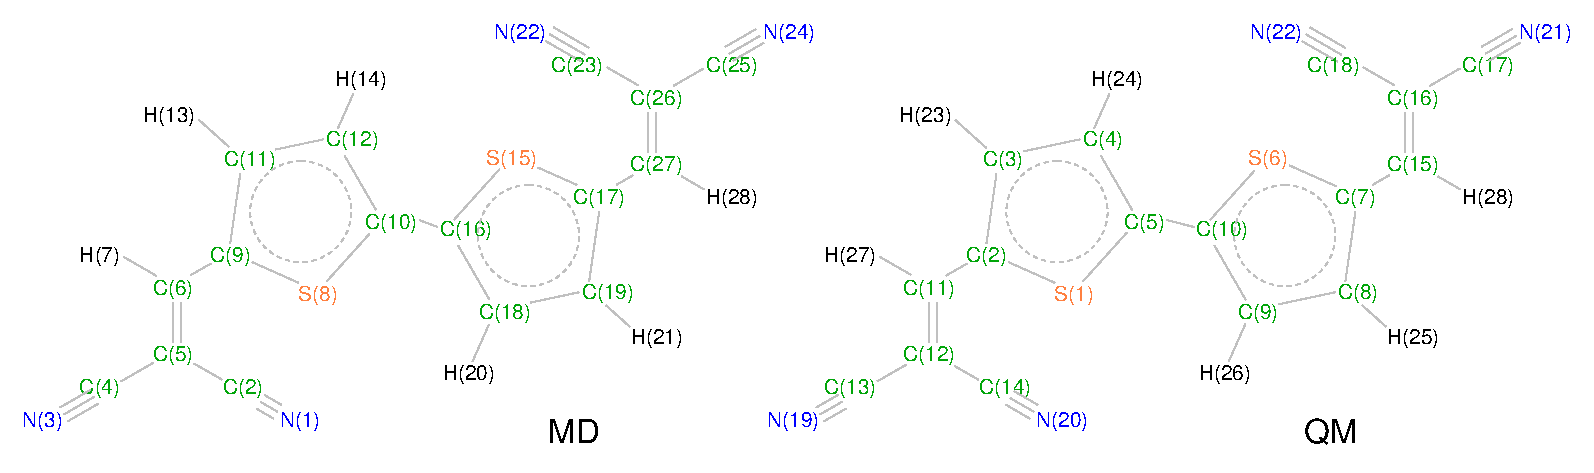
\includegraphics[width=\textwidth]{./fig/chemical_structure/dcv2t_gaussian} 
\caption{\small Atom order of \dcvt in the atomistic topology (MD) and qunatum chemical calculations (QM). The  link between two is established in the description of a conjugated segment shown in listing~\ref{list:conjugated_segments}.}
\label{fig:dcv2t_qm}
\end{figure}

\lstset{
  language=XML,
  frame=lines,
  basicstyle=\ttfamily\footnotesize,
  identifierstyle=\color{red},
  keywordstyle=\color{blue},
  showstringspaces=false,
  columns=fullflexible,
  commentstyle=\color{gray}\rmfamily\itshape,
  morekeywords={crgunit_type,ChargeUnitType,posname,orbname,basisset,transorb,reorg,nameneutr,namecrg,energy,beadconj,molname,name,monomer_atom_map,monomer_atom_weights},
}

\lstinputlisting[
 label=list:conjugated_segments, 
 caption={\small \xml file describing conjugated segments.
}]%
{./input/segments.xml}
\clearpage

%\noindent
%\suggestion{%
%crgunit\_type -> ConjugatedSegmentTypes \\ 
%ChargeUnitType -> ConjugatedSegmentType \\ 
%posname -> CoordinatesFile \\
%orbname -> OrbitalsFile \\
%transorb -> TransportOrbital \\
%reorg -> ReorganizationEnergy (do we need this here?) \\
%nameneutr -> ChargesNeutralFile \\
%namecrg -> ChargesChargedFile (do we need this here?) 
%}



\section{Molecular orbitals}
If the semi-empirical method is used to calculate electronic coupling elements, molecular orbitals of all molecules must be supplied. They can be generated using \gaussian program. The \gaussian input file for \dcvt is shown in listing~\ref{list:zindo_orbitals}. Provided with this input, \gaussian will generate \texttt{fort.7} file which contains the molecular orbitals of a \dcvt. This file can be renamed to \texttt{\dcvt.orb}. Note that the order of the atoms in the input file and the order of coefficients should always match. Therefore, the coordinate part of the input file must be supplied together with the orbitals. We will assume the coordinates, in the format \texttt{atom\_type: x y z}, is saved to the \texttt{\dcvt.xyz} file.

\lstinputlisting[
 label=list:zindo_orbitals, 
 basicstyle=\ttfamily\footnotesize,
 morekeywords={chk,mem,punch,int,S,C,S,N,H},
 showstringspaces=false,
 keepspaces=true,
 caption={\small \gaussian input file \texttt{get\_orbitals.com} used for generating molecular orbitals. The first line contains  the name of the check file, the second the requested RAM. 
%
 \texttt{int=zindos} requests the method ZINDO, \texttt{punch=mo} states that the molecular orbitals ought to be written to  the \texttt{fort.7} file, \texttt{nosymm} forbids use of symmetry and is necessary to ensure correct position of orbitals with respect to the provided coordinates. The two integer numbers correspond to the charge and multiplicity of the system: $0\, 1$ corresponds to a neutral system with a multiplicity of one. They are followed by the types and coordinates of all atoms in the molecule.
}]%
{./input/get_orbitals.com}
%


\section{Monomer calculations for DFT transfer integrals}
\lstinputlisting[
  language=XML,
  label=list:edft_gaussian_xml,
  stringstyle=\ttfamily\footnotesize,
  showstringspaces=false,
  caption={\small Example {\tt package.xml} file for the \gaussian package required in the options of the \calc{edft} \calculator for the monomer calculations as preparation for the determination of transfer integrals using \dipro.}] {./input/qmpackage_headers/gaussian_edft.xml}

\lstinputlisting[
  language=XML,
  label=list:edft_turbomole_xml,
  stringstyle=\ttfamily\footnotesize,
  showstringspaces=false,
  caption={\small Example {\tt package.xml} file for the \turbomole package required in the options of the \calc{edft} \calculator for the monomer calculations as preparation for the determination of transfer integrals using \dipro.}] {./input/qmpackage_headers/turbomole_edft.xml}

\lstinputlisting[
  language=XML,
  label=list:edft_nwchem_xml,
  stringstyle=\ttfamily\footnotesize,
  showstringspaces=false,
  caption={\small Example {\tt package.xml} file for the \nwchem package required in the options of the \calc{edft} \calculator for the monomer calculations as preparation for the determination of transfer integrals using \dipro.}] {./input/qmpackage_headers/nwchem_edft.xml}
\section{Pair calculations for DFT transfer integrals}
\lstinputlisting[
  language=XML,
  label=list:idft_gaussian_xml,
  stringstyle=\ttfamily\footnotesize,
  showstringspaces=false,
  caption={\small Example {\tt package.xml} file for the \gaussian package required in the options of the \calc{idft} \calculator for the pair calculations and the determination of transfer integrals using \dipro.}] {./input/qmpackage_headers/gaussian_idft.xml}

\lstinputlisting[
  language=XML,
  label=list:idft_turbomole_xml,
  stringstyle=\ttfamily\footnotesize,
  showstringspaces=false,
  caption={\small Example {\tt package.xml} file for the \turbomole package required in the options of the \calc{idft} \calculator for the pair calculations and the determination of transfer integrals using \dipro.}] {./input/qmpackage_headers/turbomole_idft.xml}

\lstinputlisting[
  language=XML,
  label=list:idft_nwchem_xml,
  stringstyle=\ttfamily\footnotesize,
  showstringspaces=false,
  caption={\small Example {\tt package.xml} file for the \nwchem package required in the options of the \calc{idft} \calculator for the pair calculations and the determination of transfer integrals using \dipro.}] {./input/qmpackage_headers/nwchem_idft.xml}
\section{DFT transfer integrals}
\lstinputlisting[
  language=XML,
  label=list:TI_xml,
  stringstyle=\ttfamily\footnotesize,
  showstringspaces=false,
  caption={\small Example {\tt TI.xml} file created as the output of a \dipro calculation. Due to slightly different implementations, the orbitals indices refer to monomer indices in a \gaussian run but to indices in the merged dimer guess in a \turbomole run.}] {./input/TI.xml}


\chapter{State file}
\label{sec:statefile}


\chapter{Reference}
\label{sec:reference}
\section{Programs}
\label{ref:programs}
\label{sec:programs}
Programs execute specific tasks (calculators). 

%\input{reference/programs/all}

\section{Calculators}
\label{ref:calculators}
\label{sec:calculators}

Calculator is a piece of code which computes specific system properties, such as site energies, transfer integrals, etc. \xtprun, \kmcrun are wrapper programs which executes such calculators. The generic syntax is 
\vskip 0.2cm
{\noindent \small \xtprun \exe \texttt{"calc1, calc2, ..."} \opt \xmloptions }
\vskip 0.2cm
%
File \xmloptions lists all options needed to run a specific calculator. The format of this file is explained in listing~\ref{list:calc}. A complete list of calculators is given in the \refcalc reference section.
%
\lstinputlisting[label=list:calc, 
 caption={\small A part of the \xmloptions file with options for the \texttt{calculator\_name\{1,2\}} \refcalc.
}]{./reference/calculators.xml}

A list of all calculators and their short descriptions can be obtain using 
\vskip 0.1cm
{\noindent \small \xtprun \texttt{-{}-list} }
\vskip 0.1cm

A detailed description of all options of a specific calculator(s) is available via
\vskip 0.1cm
{\noindent \small \xtprun \texttt{-{}-desc calc1,calc2,...} }

%\subsection{Calculators}
\label{sec:calculators}

Calculator is a piece of code which computes specific system properties, such as site energies, transfer integrals, etc. \ctprun is a wrapper program which executes all calculators. The generic syntax is 
\begin{verbatim}
  ctp_run --exec "calc1, calc2, ..." --opt options.xml
\end{verbatim}
%
File \texttt{options.xml} lists all options needed to run a specific calculator. The format of this file is explained in listing~\ref{list:calc}. A complete list of calculators is given in the \refcalc reference section.
%
\lstinputlisting[label=list:calc, 
 caption={\small A part of the \texttt{options.xml} file with options for the \texttt{calculator\_name\{1,2\}} \refcalc.
}]{./programs/calculators.xml}

\vfill

\section{Common options}
\label{ref:options}
%\setdefaultleftmargin{0.8em}{0.8em}{0.8em}{0.8em}{0.8em}{0.8em}
\rowcolors{1}{invisiblegray}{white}
{\small 
%\input{reference/xml/options.xml}
}
\vfill


%\appendix
%\input{appendix/xtp_standalone}

\nolinenumbers

\bibliographystyle{short}
{\footnotesize \bibliography{literature_short} }

\end{document} 
